\chapter{Novel Dataset Class}
\label{chap:datasets}

This chapter introduces the novel dataset category representing a flat connector. The sections will revolve mainly around the specifics of the flat connector object, the setup used to 
record the data and produce labels, as well as the anomalies chosen for this class. Section \ref{sec:flatconnectoranomalies} also reviews the steps to produce the specific anomalies 
and how to recreate them.


\section{Flat Connector}
\label{sec:faltconnectordesscription}

As mentioned prior to this chapter, this work will also deal with the introduction of a novel dataset category that is an extension of the MVTecAD LOCO \cite{LOCODentsAndScratchesBergmann2022} dataset. 
Despite simply extending the range of objects covered in the dataset, this also serves as a more varied investigation of IAD method performance in industrial settings. The motivation behind adhering 
to MVTecAD LOCO standards is multifold. Firstly, the setting of this work is already in the context of logical anomalies, which greatly facilitates the evaluation of the new class. Additionally, as 
discussed in section \ref{sec:datasets}, there is only a slight technical difference between the MVTecAD LOCO and the classical MVTecAD \cite{MVTEC_Bergmann_2021} dataset, meaning that this novel 
class can easily be evaluated by most IAD approaches, as most already report their performance on the MVTecAD dataset. This holds true for past approaches but also new ones 
to come.
\newline\newline
The flat connector object was chosen since it meets multiple requirements for an adequate object class. It is of a metal manufacturing nature and can comfortably be photographed from 
an overhead perspective. Although the MVTecAD LOCO dataset already contains a screw bag, the property of the plastic bag could potentially shift the focus of the performance from solely the metal 
part performance to the anomaly localization in more difficult conditions. The latter is a common characteristic of the other classes in the set. Finally, the flat connector has some 
properties that make it a very favorable manufacturing part include the following: It is of lighter metal, giving us much more freedom to produce anomalies. A steel block, for example, would be vastly 
harder to meaningfully process into it, representing various kinds of anomalies. Moreover, the differently sized holes in set configurations that the flat connector possesses make for many opportunities 
to introduce logical anomalies without the need for arbitrary rules like the pushpin or splicing connector class. For example, the latter class may need multiple objects in a certain arrangement per image to then predefine 
rules as logical constraints, whereas the flat connector, as such, may possess multiple logical violations within only one object without the need for additional artificial rules.
\newline
Further, regarding the flat size specifications, we used regulatory flat 
connectors of size $100x35 mm$ which are widely available at hardware stores and at \cite{flatconnectorlink}. The surface of the flat connectors is galvanized 
and displays a CE label according to DIN EN 14545. Images of normal flat connectors without manipulations can be viewed in appendix Fig. \ref{fig:flatgoodimages}.




\begin{figure}[ht]
    \captionsetup[subfigure]{justification=centering}
    \centering
    \begin{subfigure}[b]{0.3\textwidth}
        \centering
        \includegraphics[width=0.475\textwidth]{figures/flatconnectordatasetimages/cut_corner_image.png}
        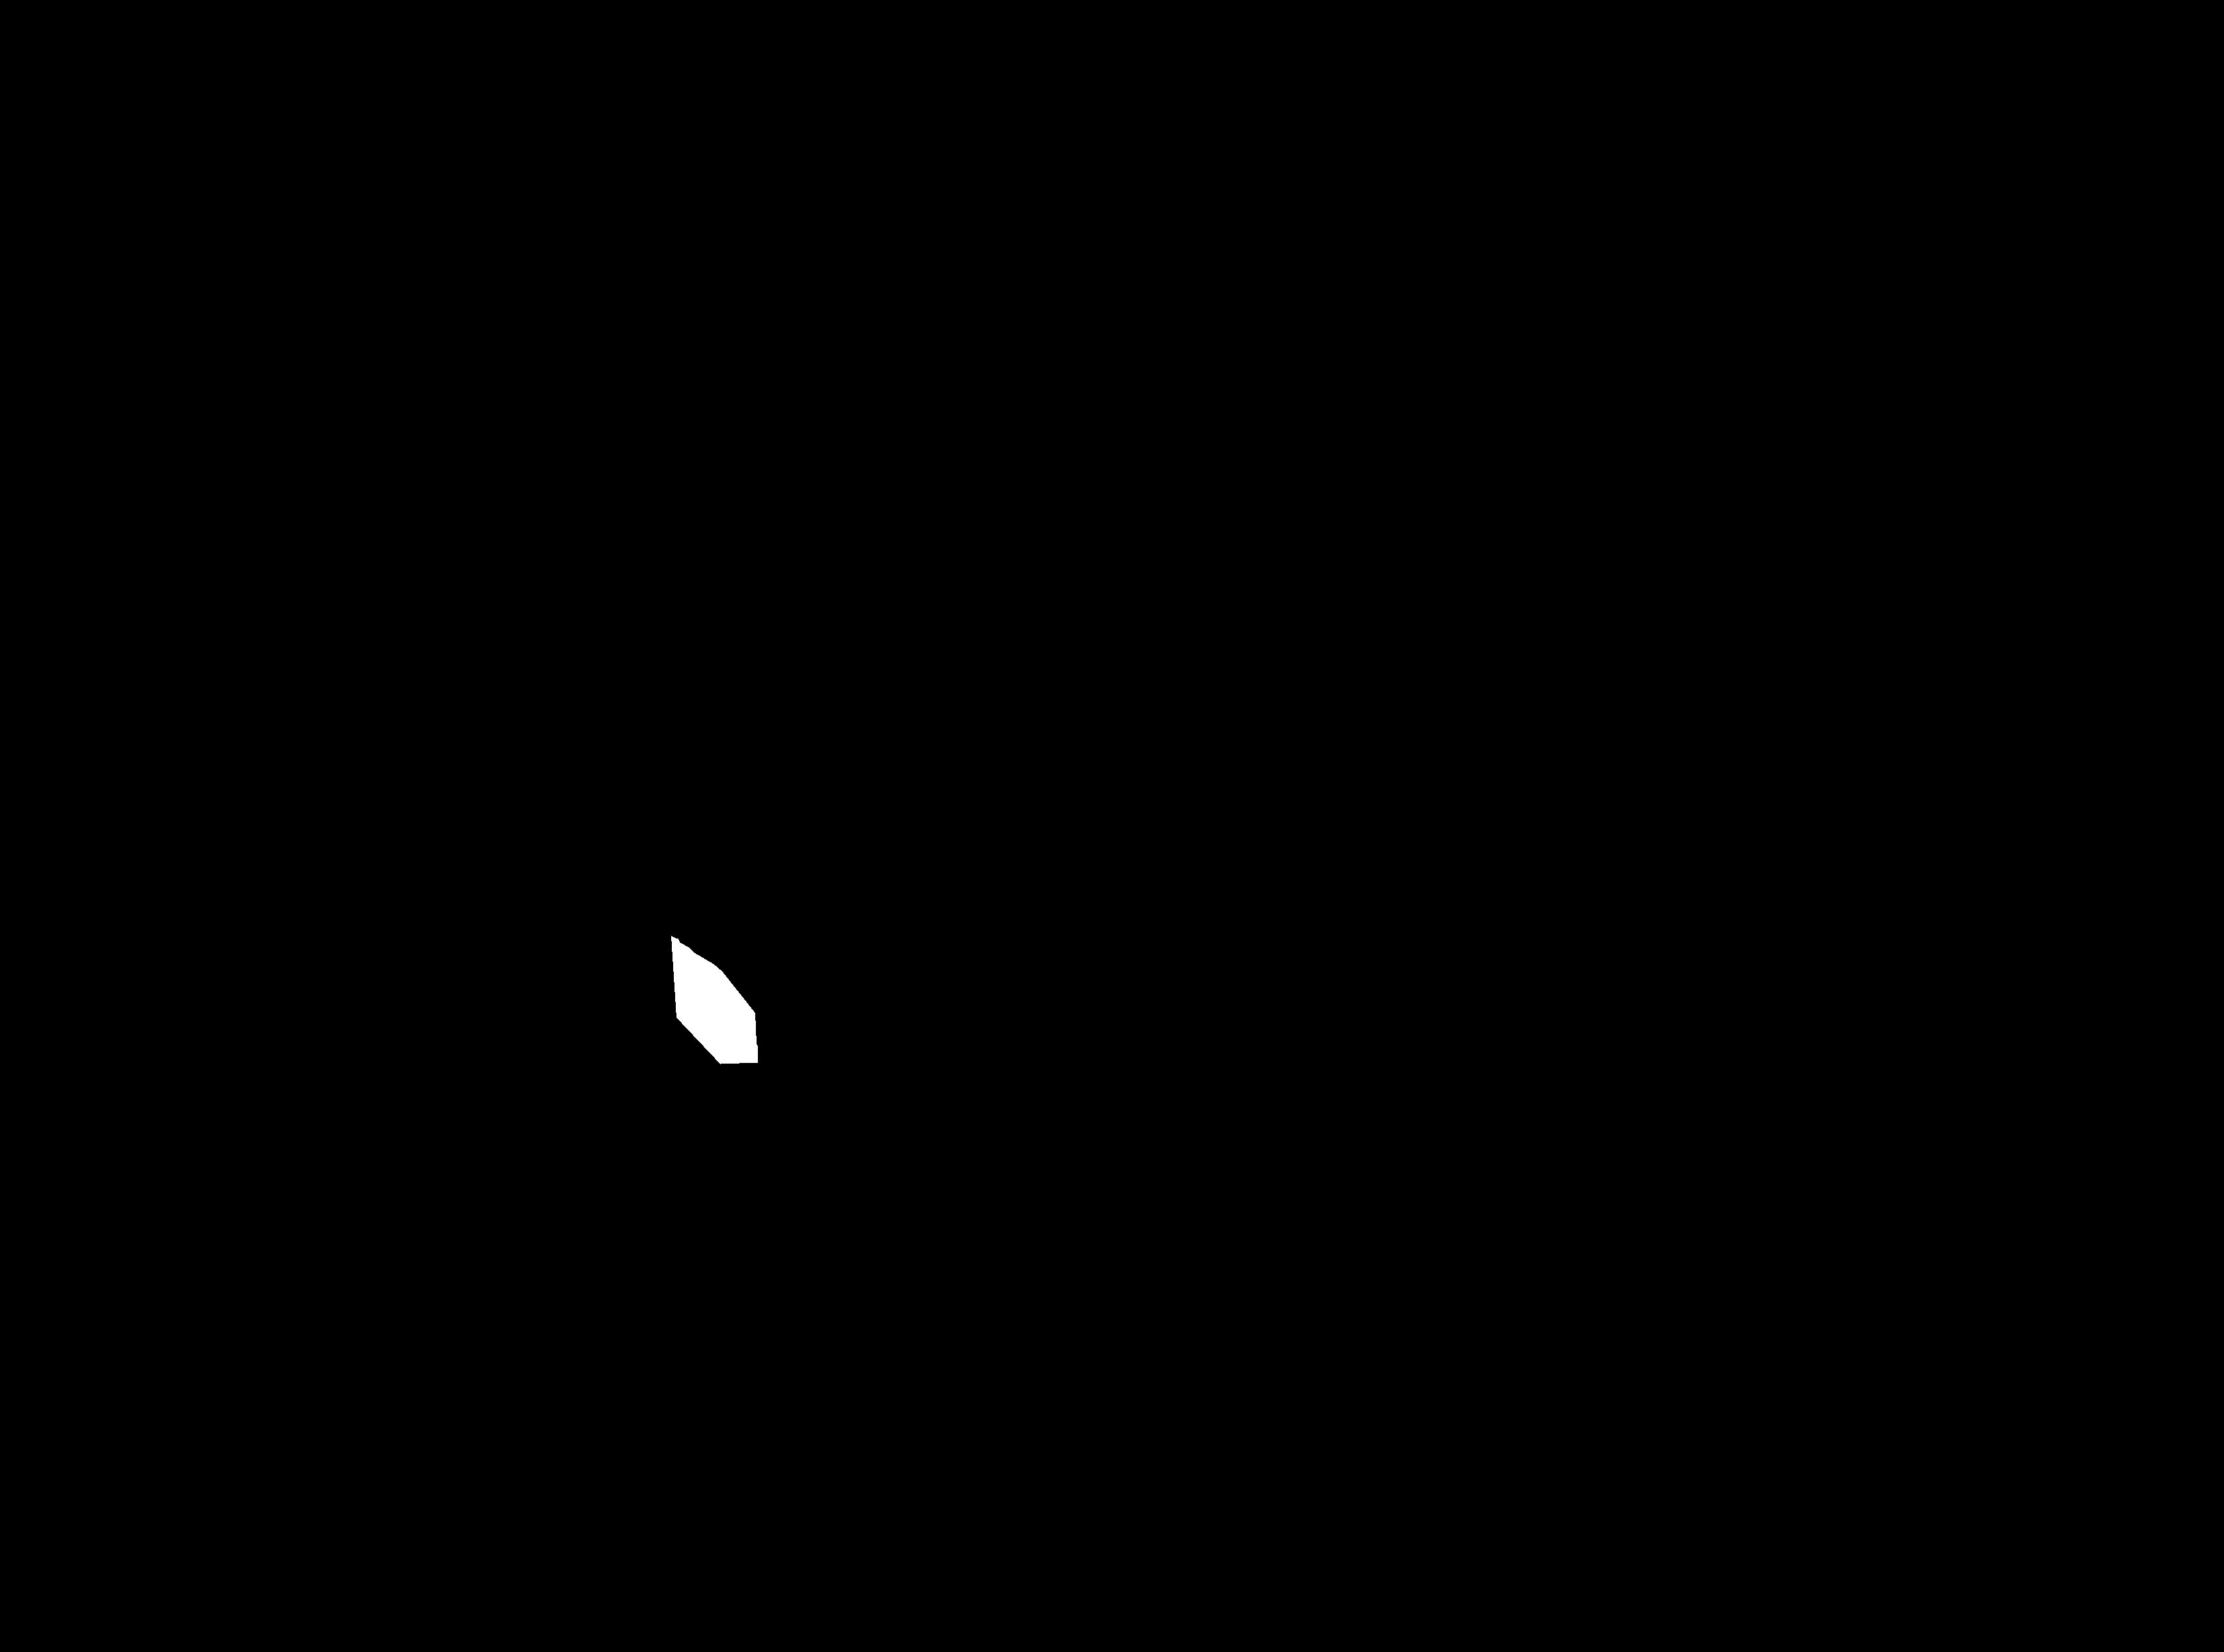
\includegraphics[width=0.475\textwidth]{figures/flatconnectordatasetimages/cut_corner_mask.png}
        \caption*{Cut Corner}

    \end{subfigure}
    \hfill
    \begin{subfigure}[b]{0.3\textwidth}
        \centering
        \includegraphics[width=0.475\textwidth]{figures/flatconnectordatasetimages/damaged_edge.png}
        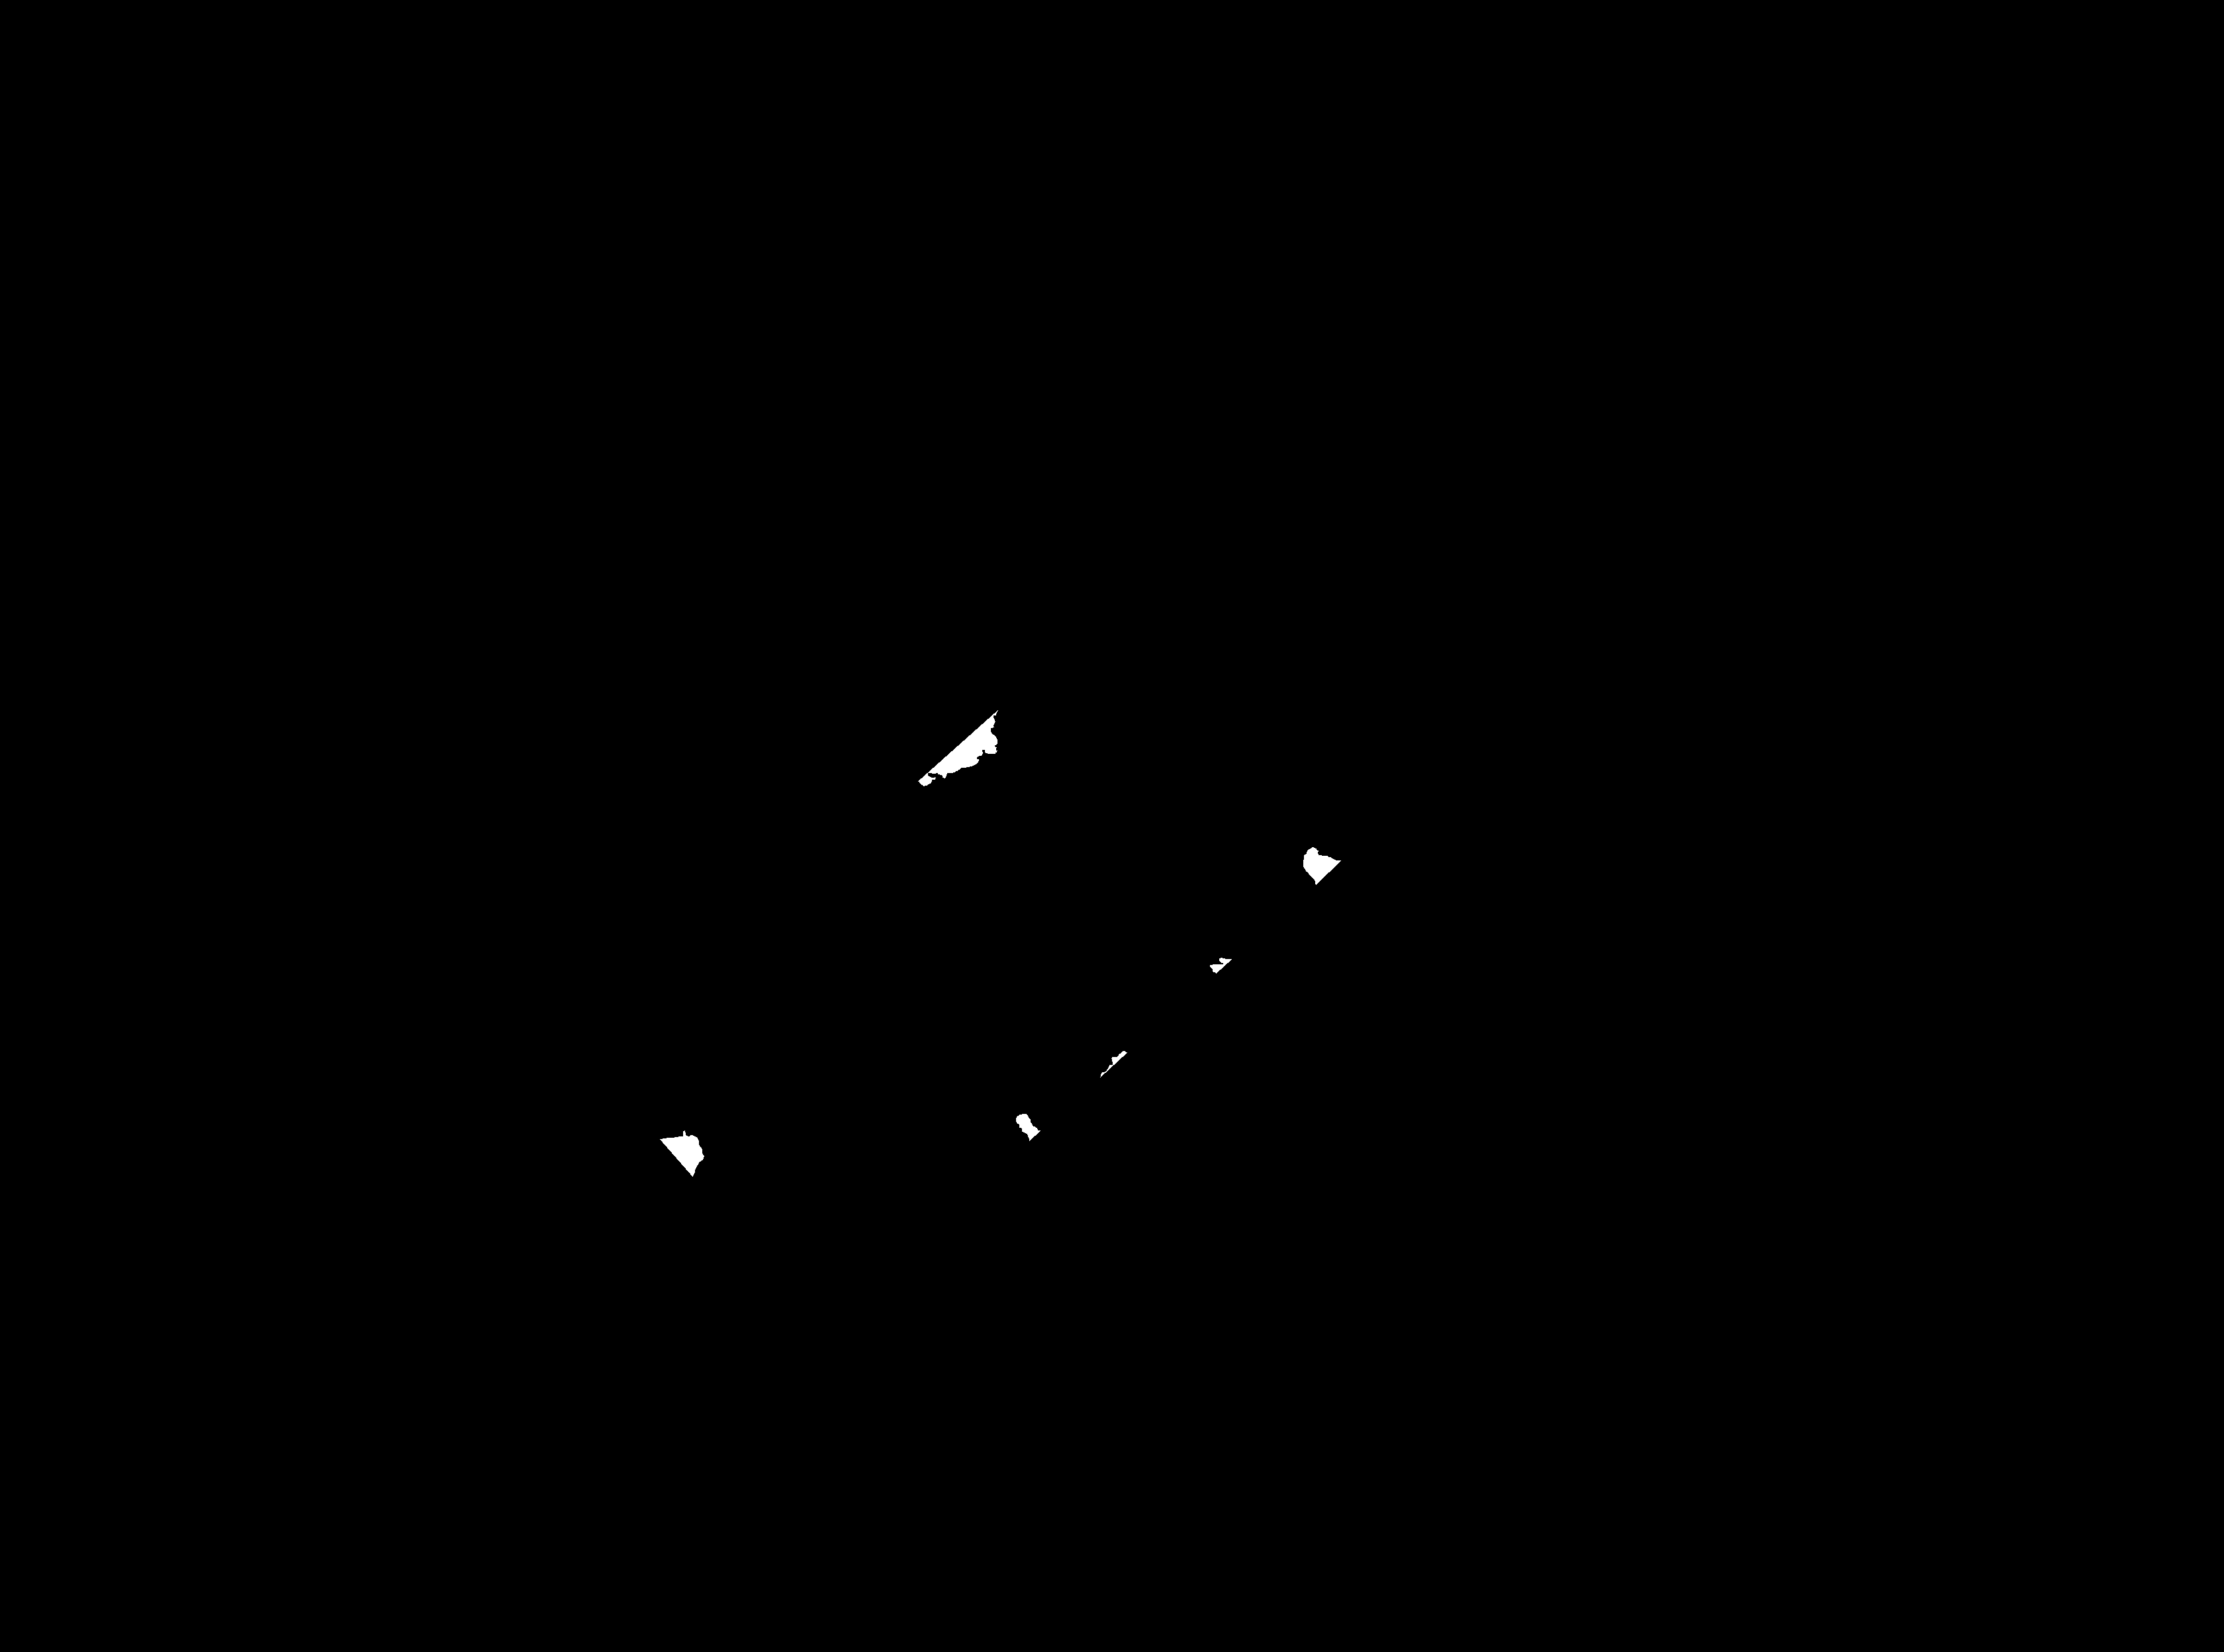
\includegraphics[width=0.475\textwidth]{figures/flatconnectordatasetimages/damaged_edge_mask.png}
        \caption*{Damaged Edge}

    \end{subfigure}
    \hfill
    \begin{subfigure}[b]{0.3\textwidth}
        \centering
        \includegraphics[width=0.475\textwidth]{figures/flatconnectordatasetimages/scratch.png}
        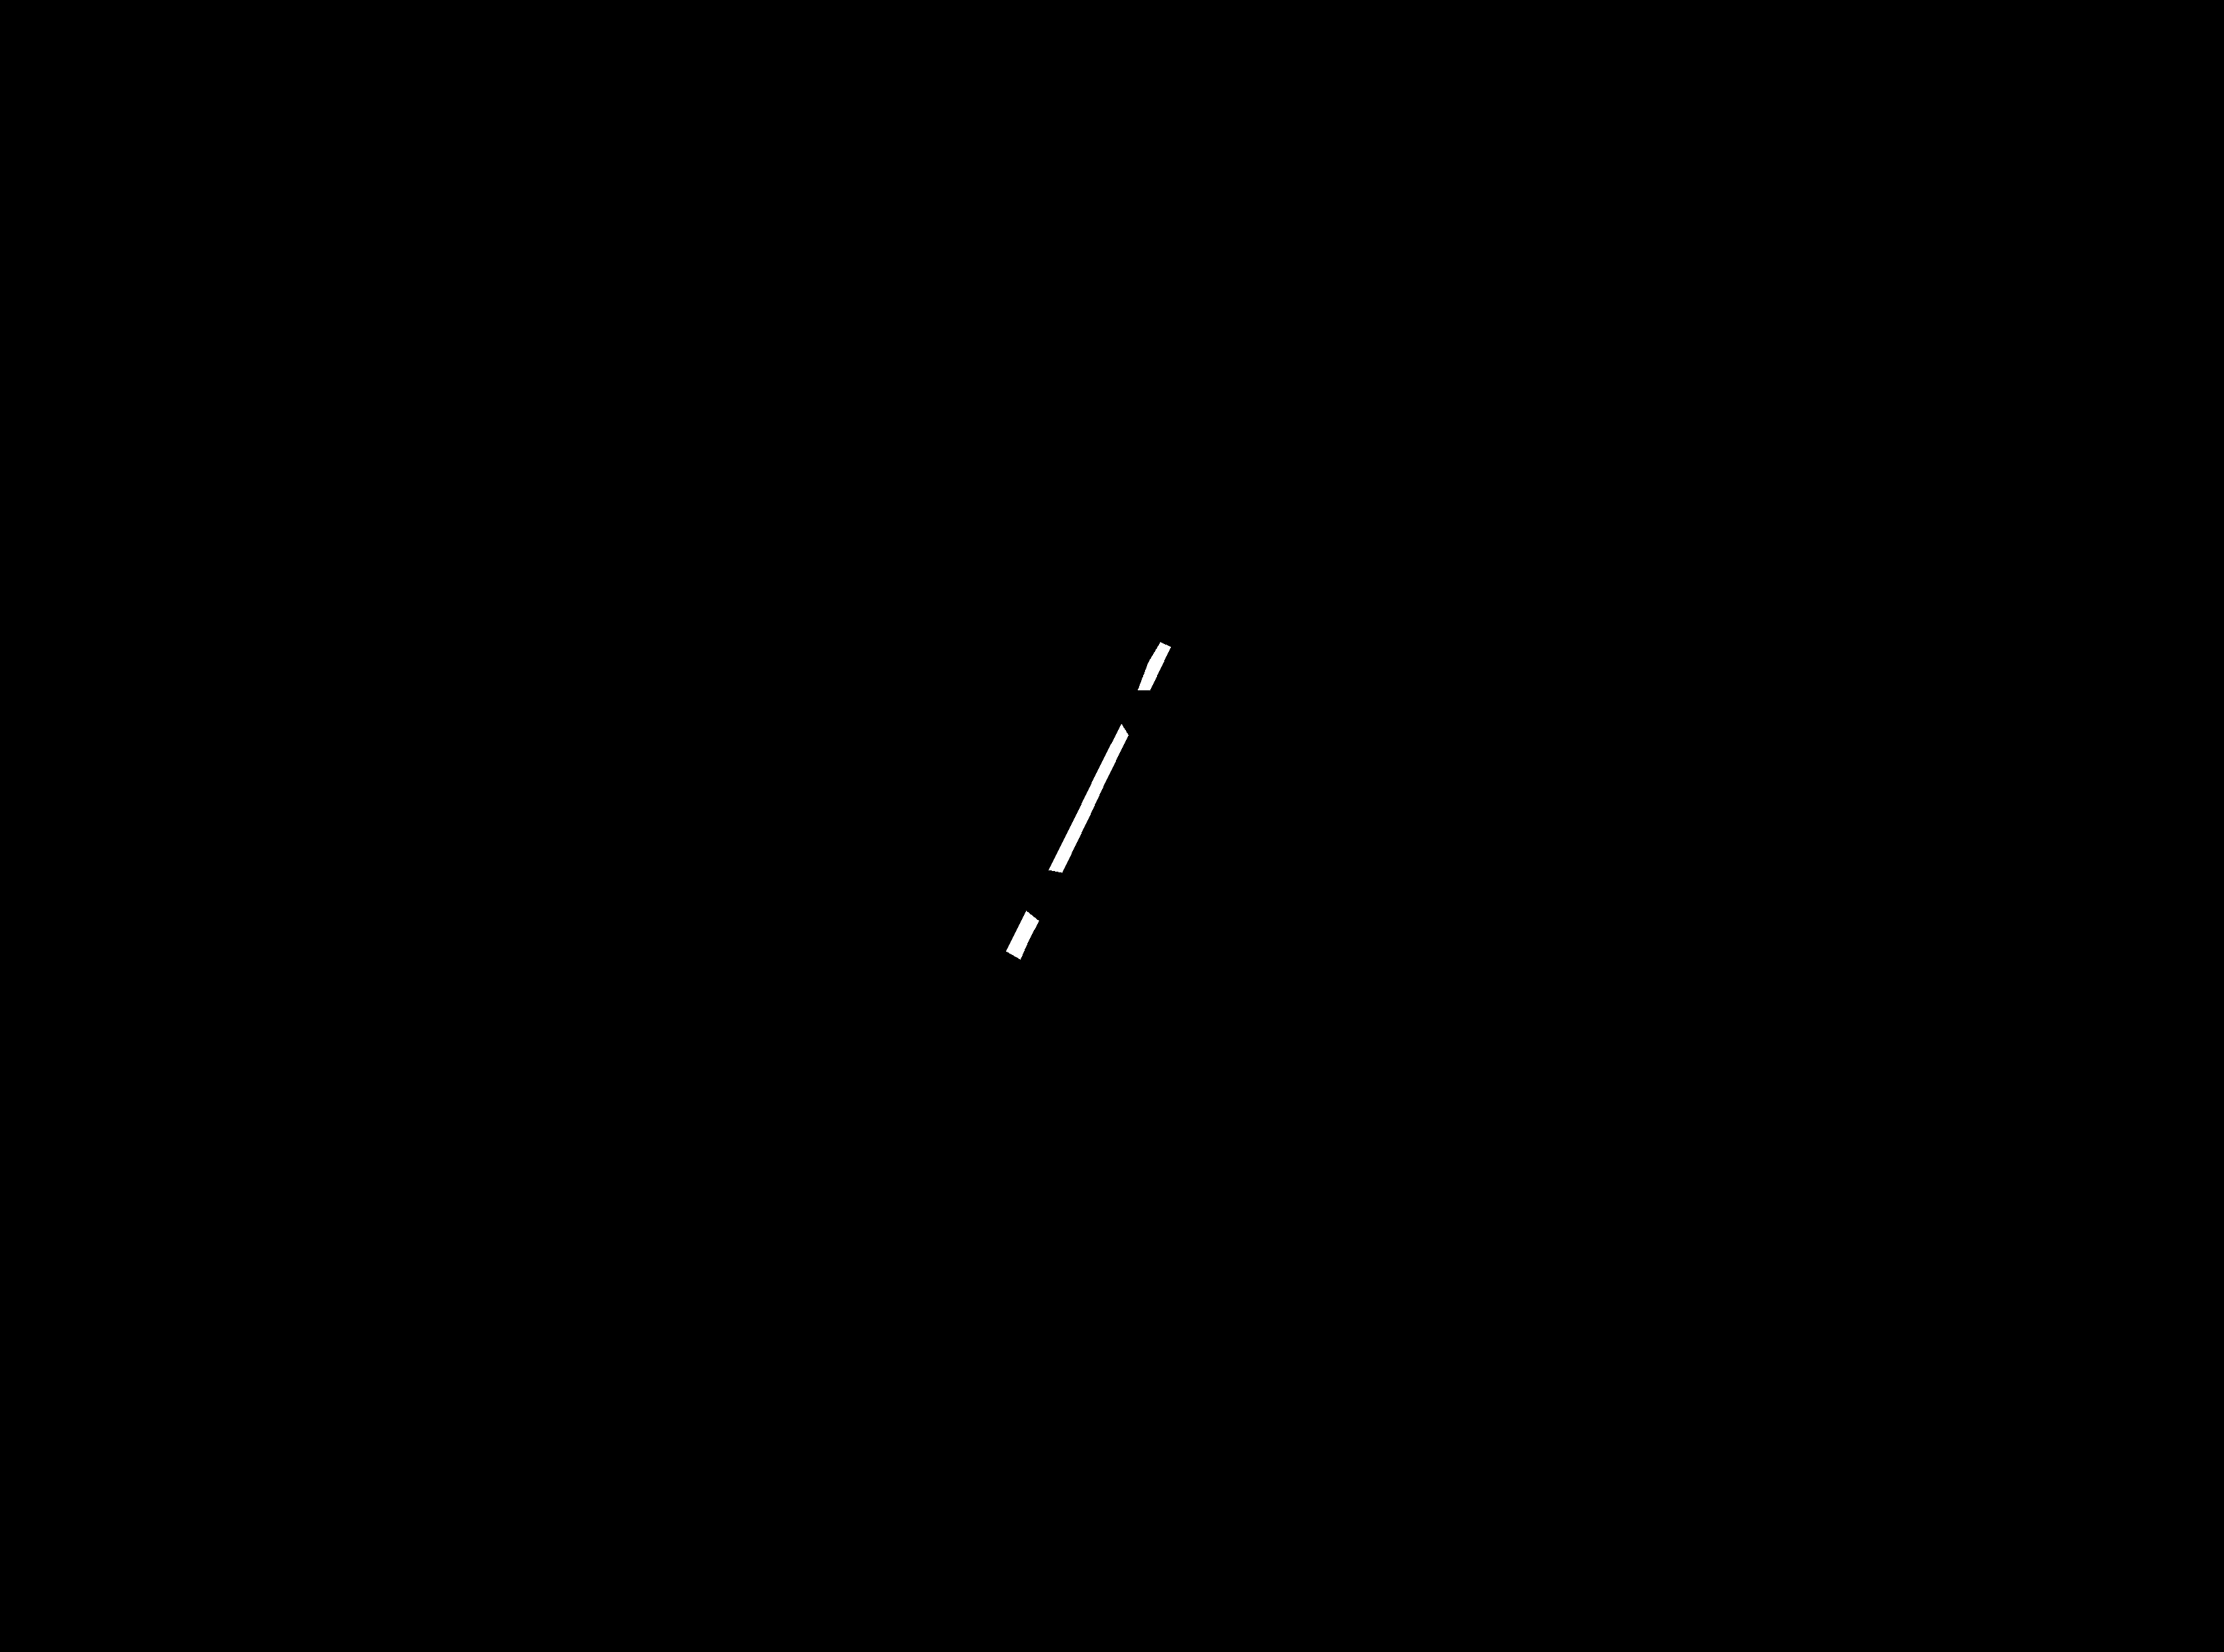
\includegraphics[width=0.475\textwidth]{figures/flatconnectordatasetimages/scratch_mask.png}
        \caption*{Scratch}

    \end{subfigure}
    \\
    \begin{subfigure}[b]{0.3\textwidth}
        \centering
        \includegraphics[width=0.475\textwidth]{figures/flatconnectordatasetimages/missing_big_hole.png}
        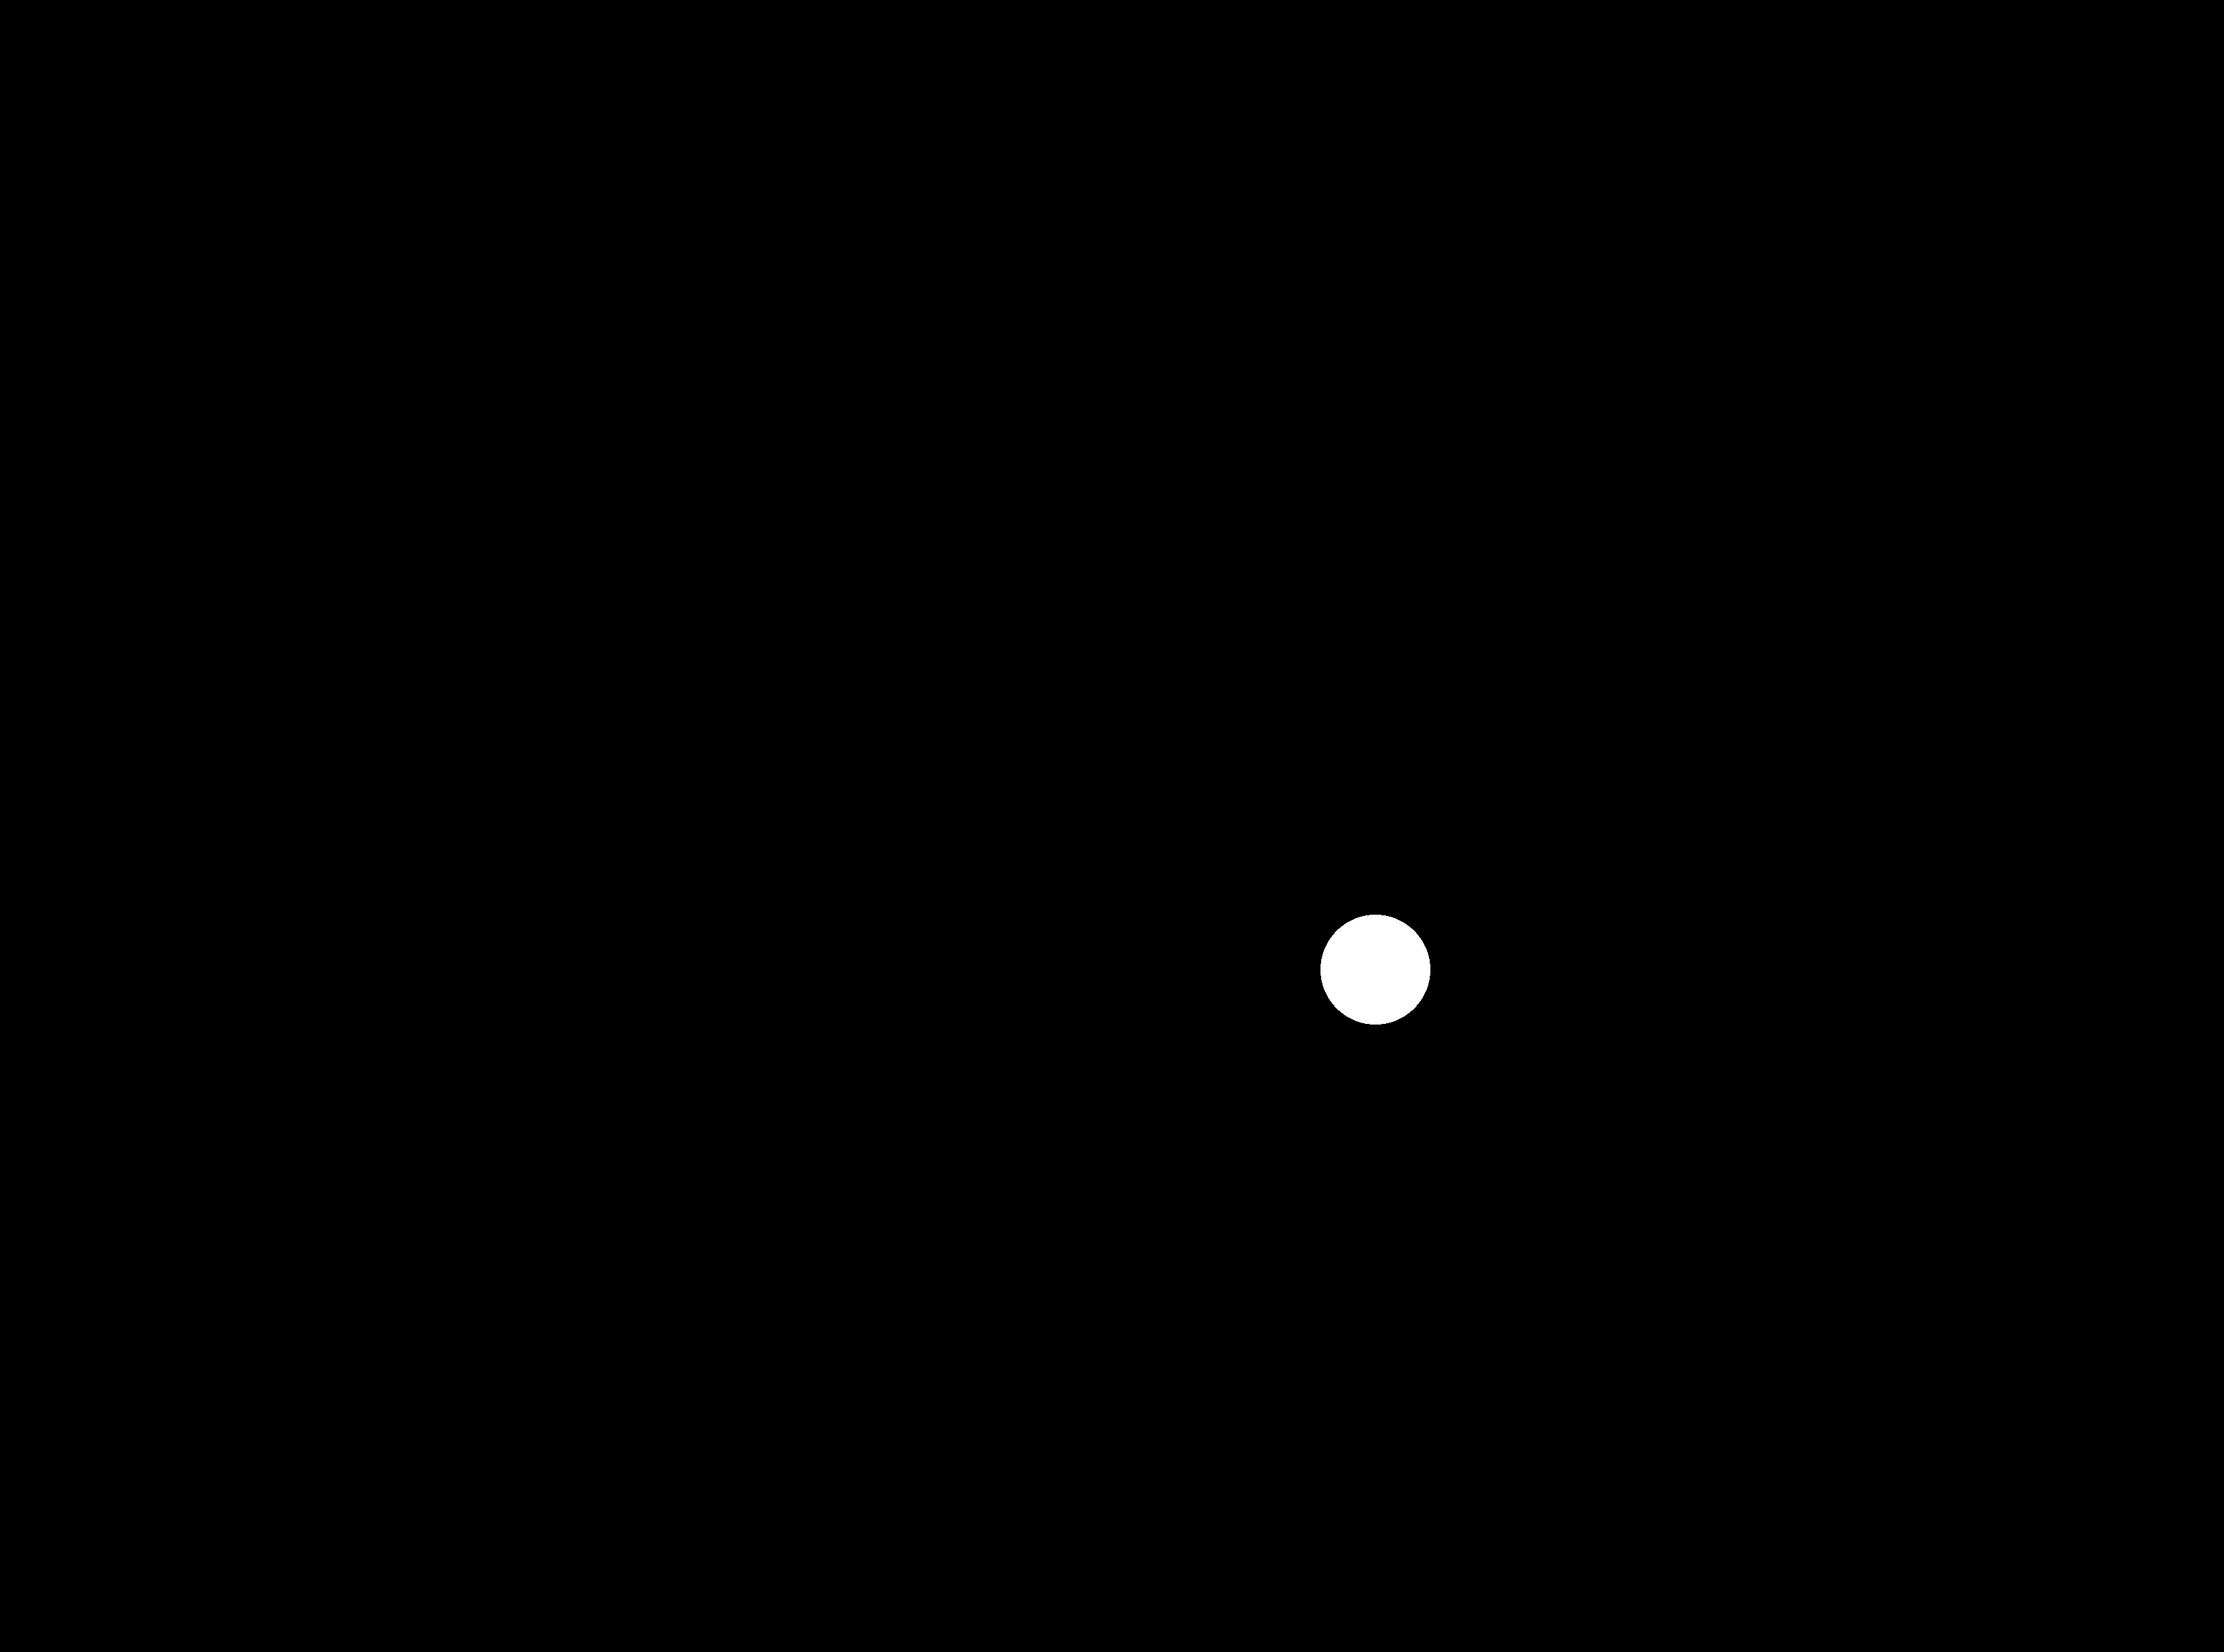
\includegraphics[width=0.475\textwidth]{figures/flatconnectordatasetimages/missing_big_hole_mask.png}
        \caption*{Missing Big Hole}

    \end{subfigure}
    \hfill
    \begin{subfigure}[b]{0.3\textwidth}
        \centering
        \includegraphics[width=0.475\textwidth]{figures/flatconnectordatasetimages/extra_holes.png}
        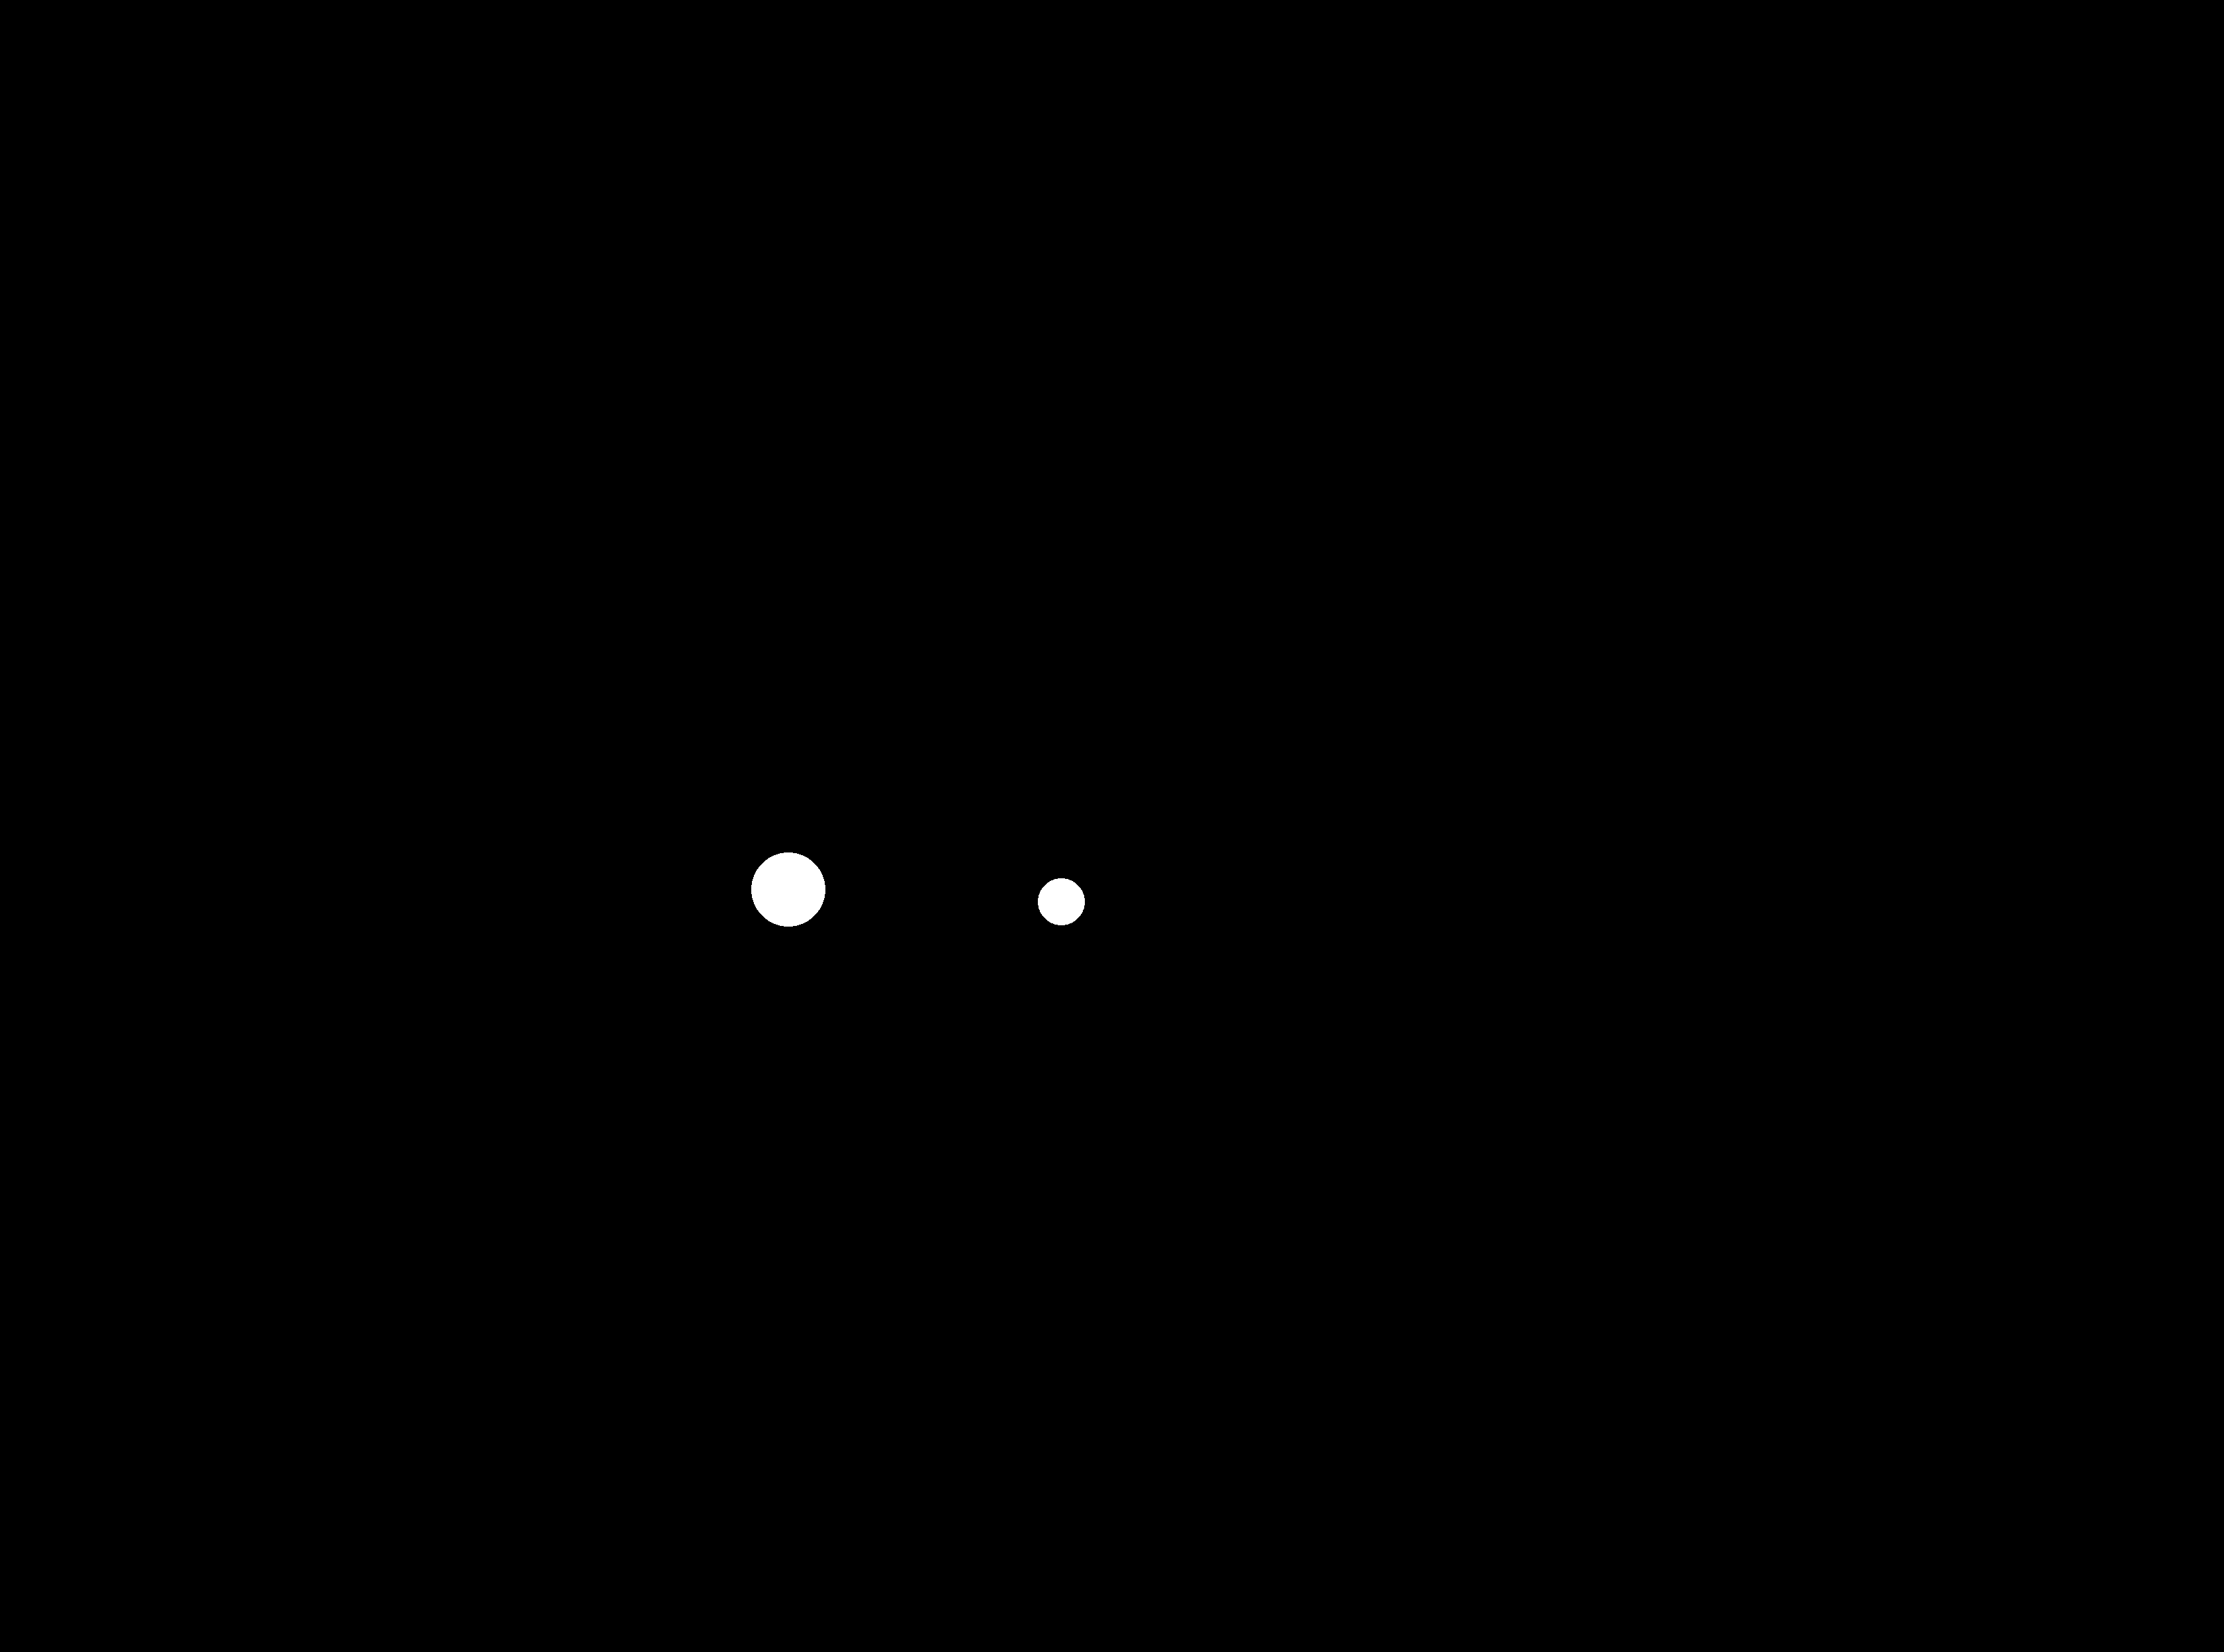
\includegraphics[width=0.475\textwidth]{figures/flatconnectordatasetimages/extra_holes_mask.png}
        \caption*{Extra Holes}

    \end{subfigure}
    \hfill
    \begin{subfigure}[b]{0.3\textwidth}
        \centering
        \includegraphics[width=0.475\textwidth]{figures/flatconnectordatasetimages/diff_size_holes.png}
        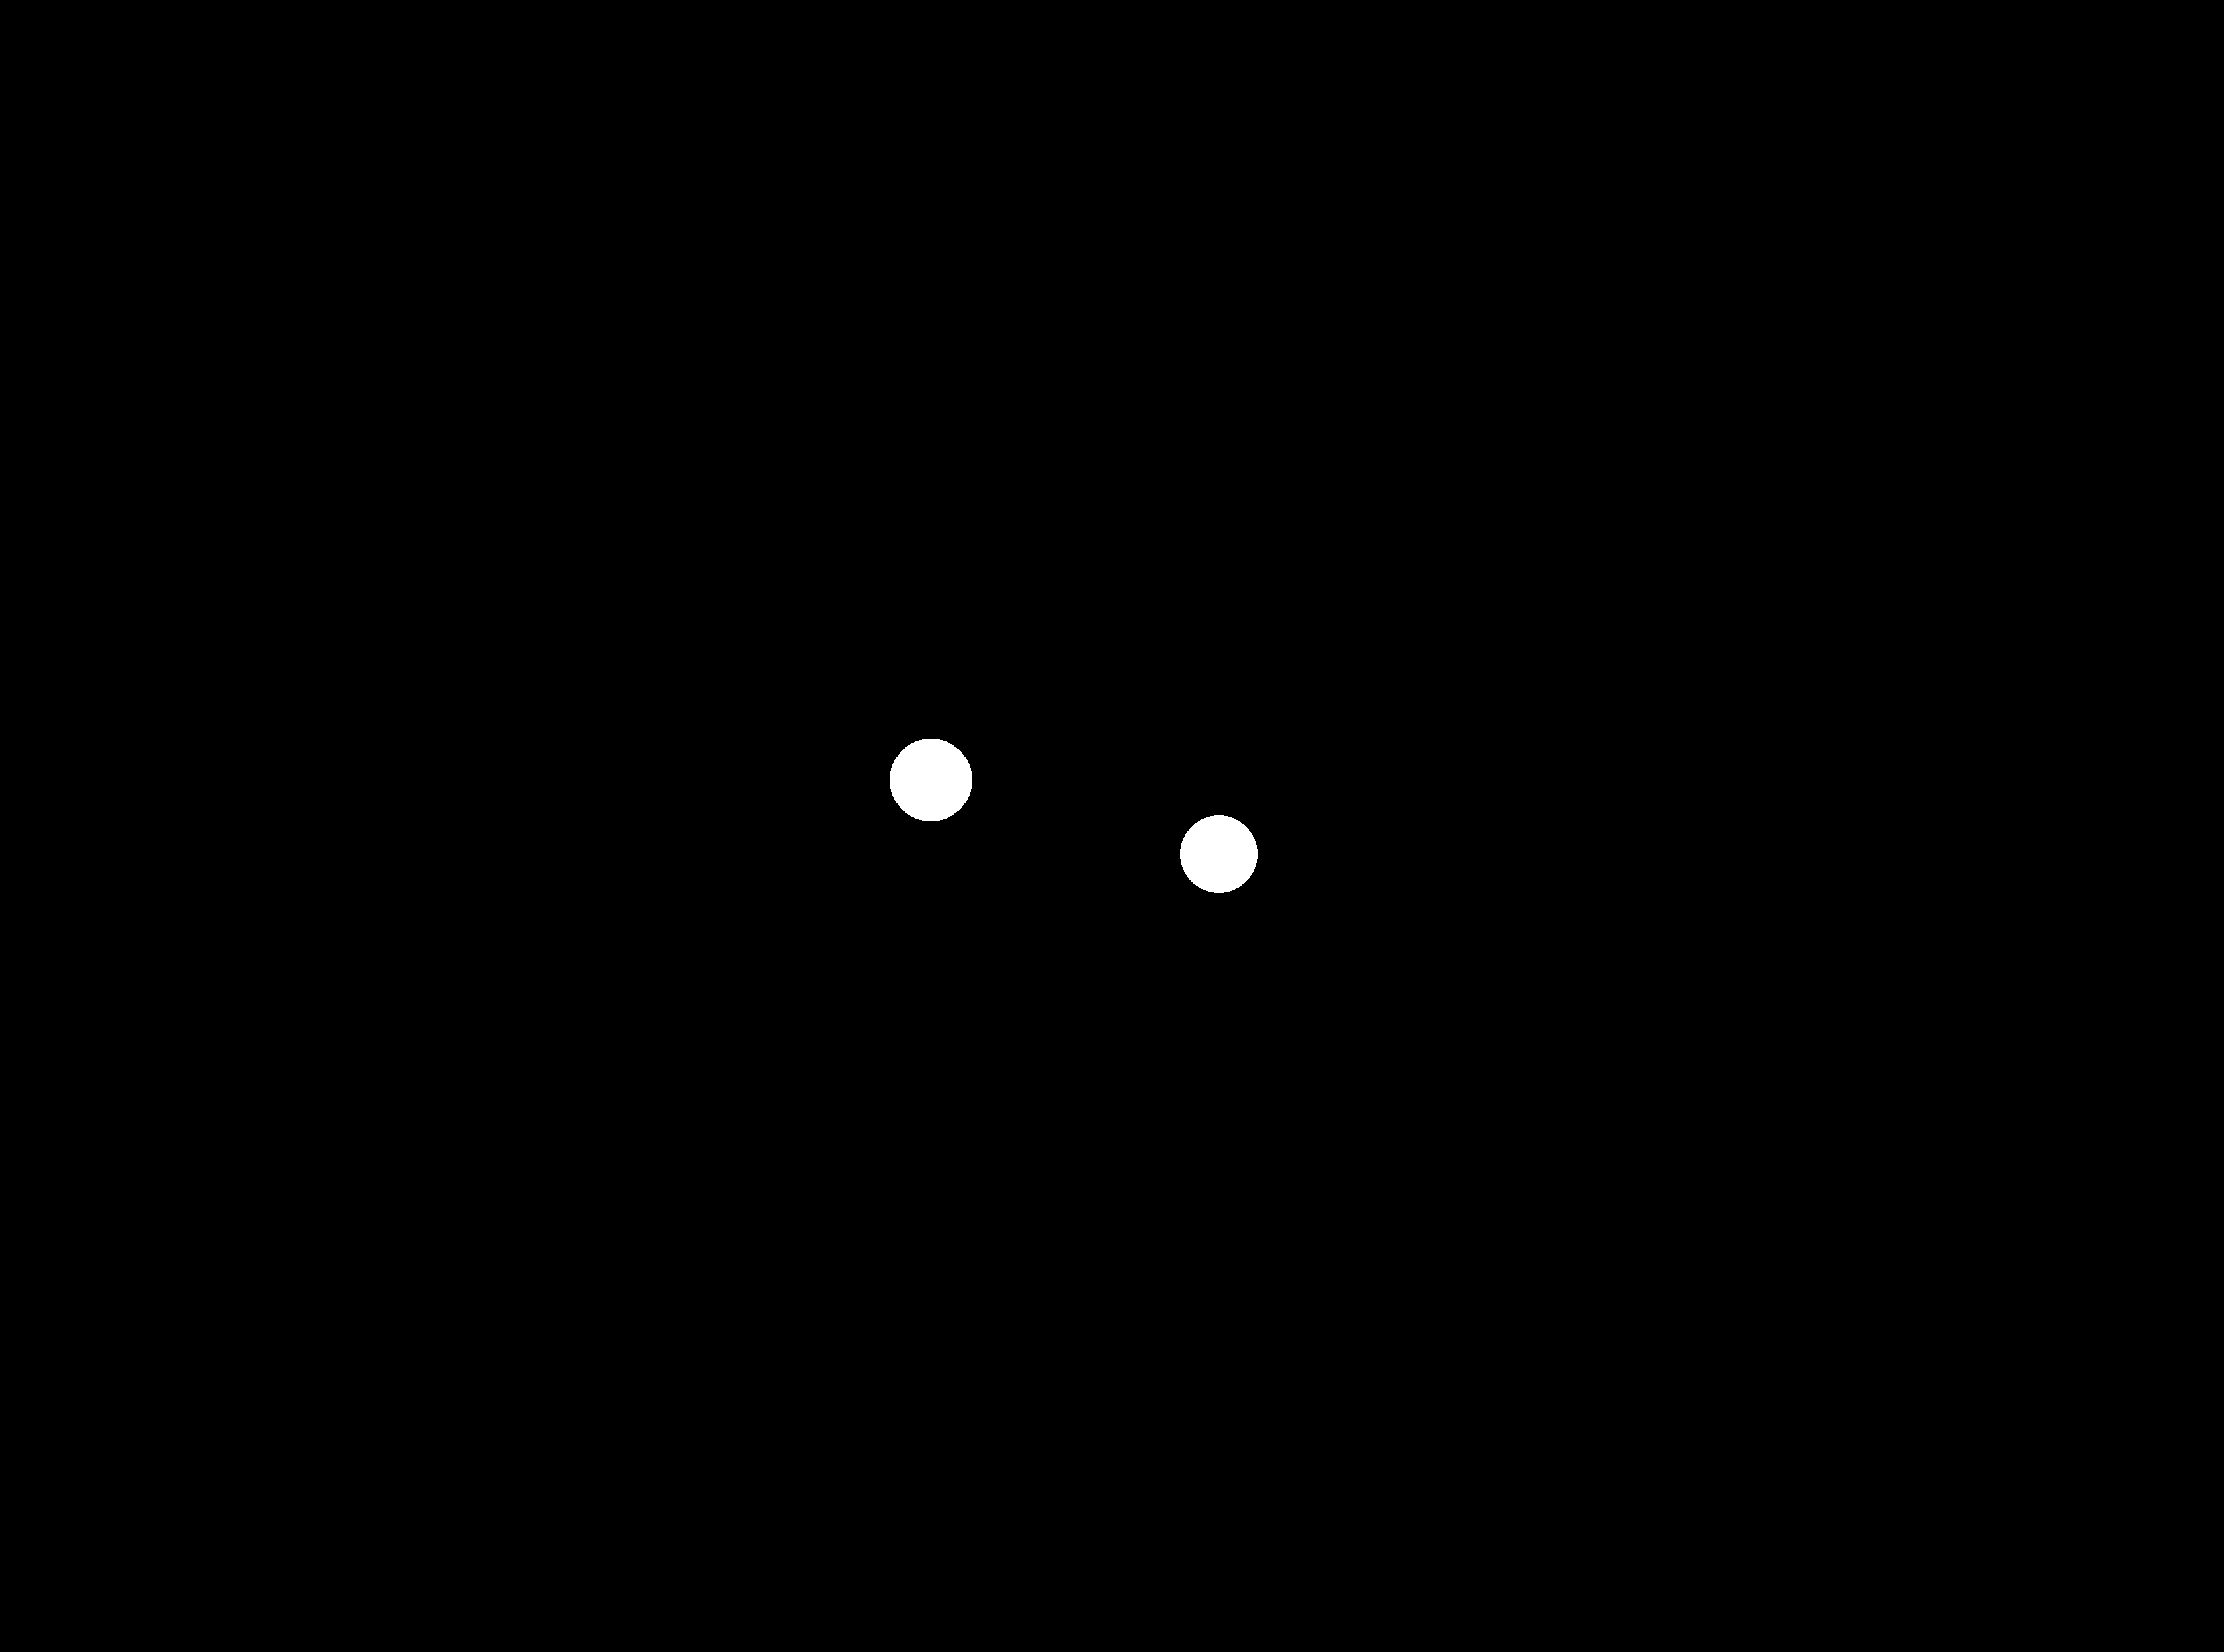
\includegraphics[width=0.475\textwidth]{figures/flatconnectordatasetimages/diff_size_holes_mask.png}
        \caption*{Differently Sized Holes}

    \end{subfigure}
    %\captionsetup{justification=centering, skip=-10pt}
    \caption{Anomalous Flat Connector Images and the Corresponding Masks}
    \label{fig:flatconnectorexampleimages}
\end{figure}






\section{Data Acquisition Setup}
\label{sec:faltconnectordataacquisiton}

The images for the dataset were taken at university facilities.  Fig. \ref{fig:setupofdatacollection} shows an exemplary setup for image acquisition. The contraption to capture images was 
done by utilizing a camera mounted to a robotic arm and pointing the camera lens at the table from an overhead perspective. The distance between the camera lens and the table surface was approximately 15 cm and the main light source for the images was provided by a built-in flashlight of the arm. Regarding the object's background, a black cloth was placed on the table where the object would be put. For 
an increased variety, multiple flat connectors were bought and filmed. Here, each one was manually rotated after each shot to achieve multiple object orientations and, thus, a more robust training 
set. Each flat connector was rotated six times per side, resulting in 12 normal images per flat connector object. \newline
The camera used to take pictures produced the images of the flat connectors in a 4k resolution. Due to the large size of the resulting 
images, their size was adjusted by half of the original image size.\newline
A free polygon annotation software was used to label anomalous regions in the images to obtain segmentation labels. The annotations were done by hand and by the author of this work. In accord with 
MVTecAD LOCO standards \cite{LOCODentsAndScratchesBergmann2022}, each kind of anomaly would be assigned a unique pixel value to differentiate them when working with saturation thresholds 
as mentioned in section \ref{sec:datasets}. Example annotations can be viewed in Fig. \ref{sec:flatconnectoranomalies}, where several original images are depicted next to the produced segmentation labels. Just like in the 
original MVTecAD LOCO dataset, image labels were not explicitly given since they can be inferred by the anomaly class.


\begin{figure}[htbp]
    \captionsetup[subfigure]{justification=centering}
    \centering
    \begin{subfigure}[b]{0.3\textwidth}
        \centering
        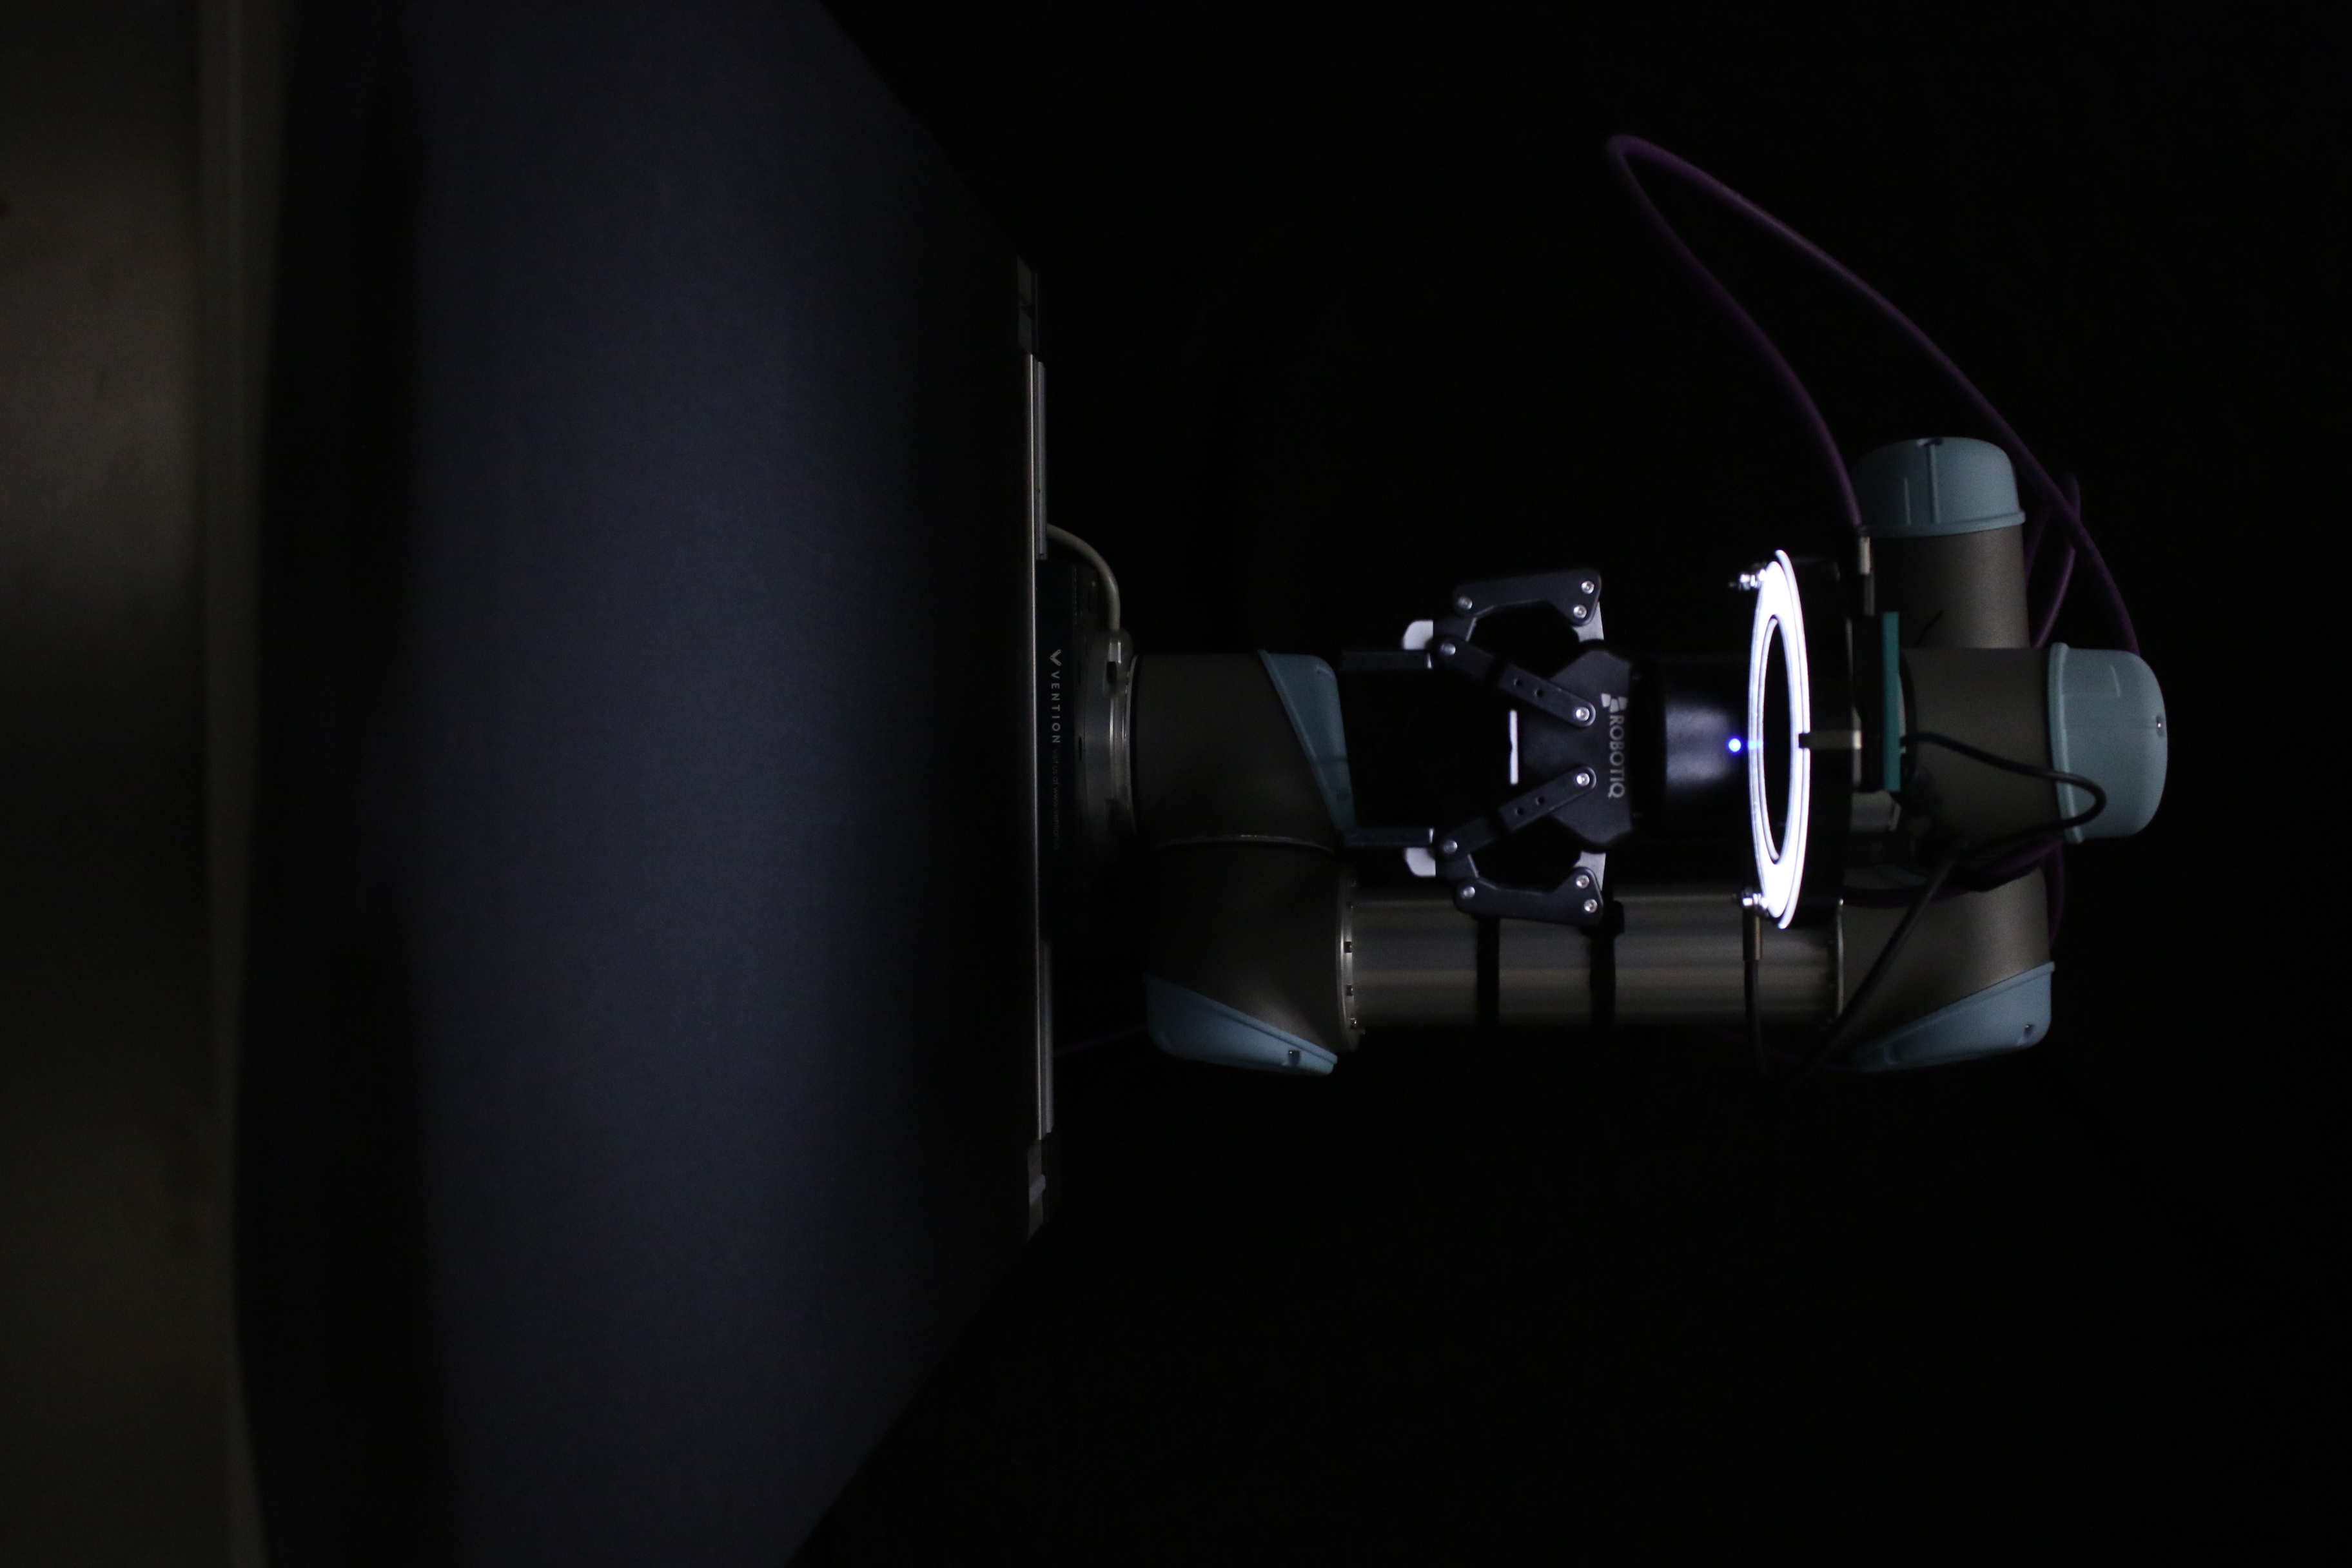
\includegraphics[angle=90, width=\textwidth]{figures/setupimages/setup_empty.JPG}


    \end{subfigure}
    \begin{subfigure}[b]{0.3\textwidth}
        \centering
        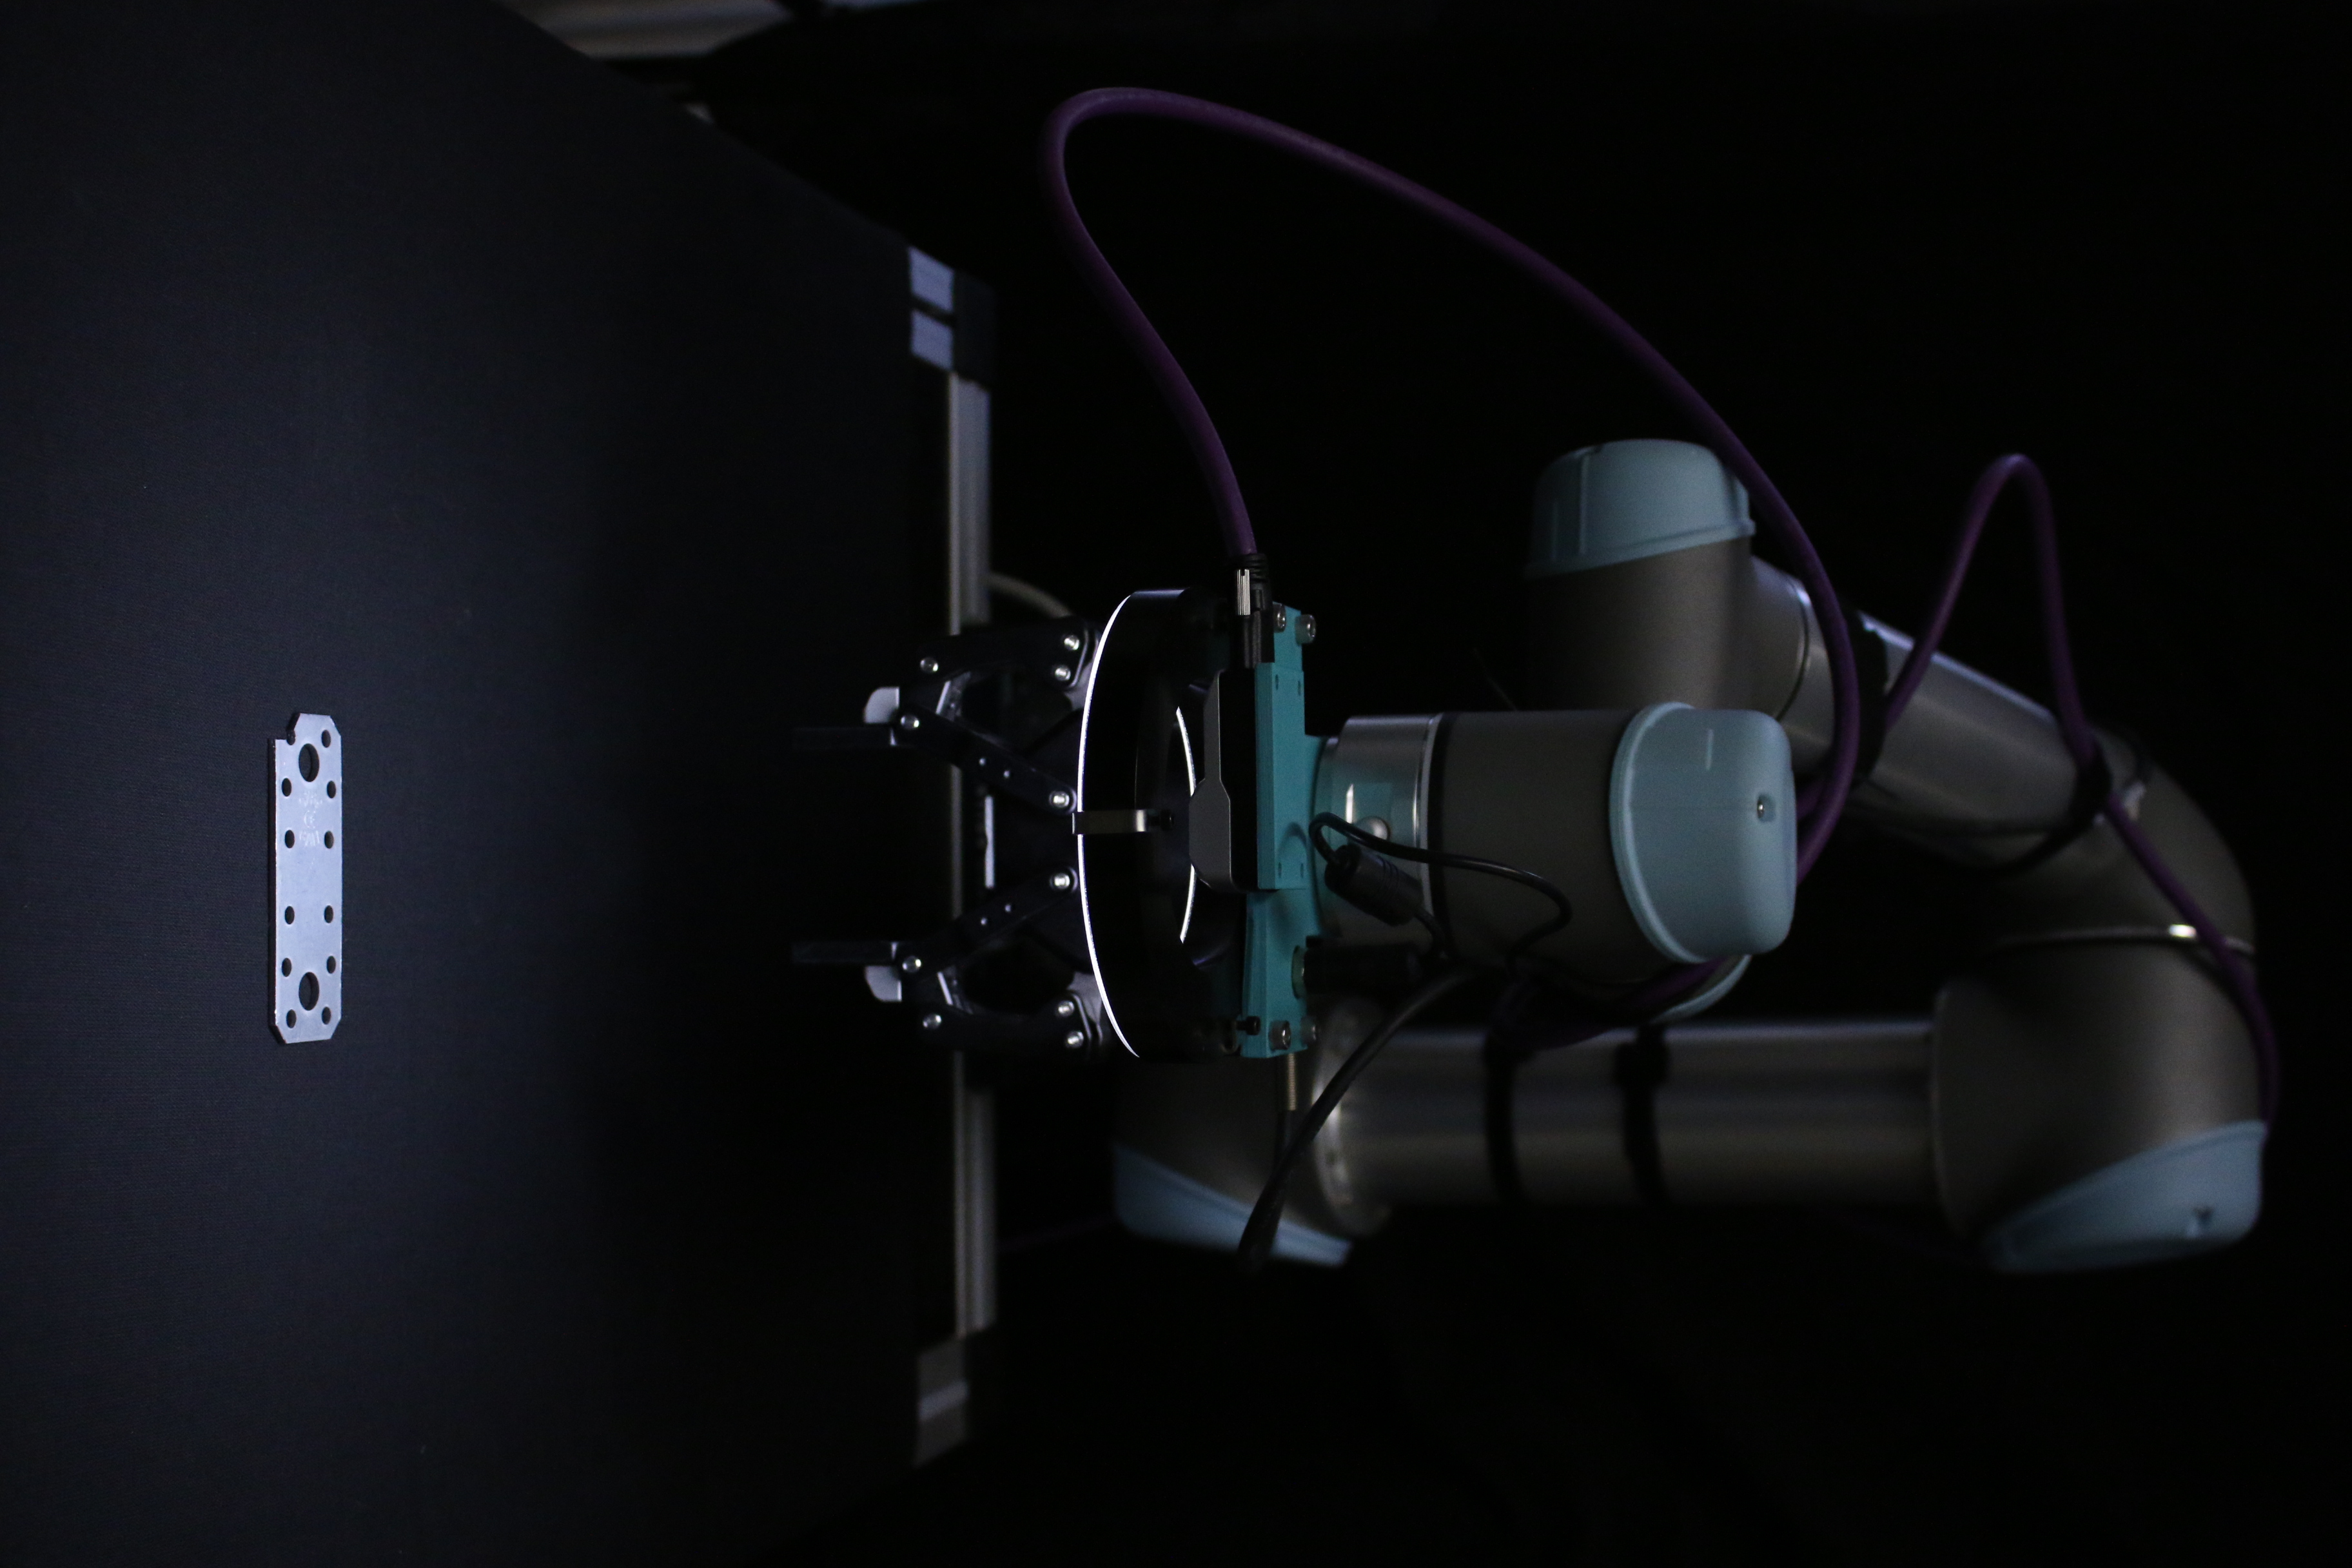
\includegraphics[angle=90, width=\textwidth]{figures/setupimages/setup_flachverbinder.JPG}
        %\caption*{Logical Anomalies}

    \end{subfigure}
    \begin{subfigure}[b]{0.3\textwidth}
        \centering
        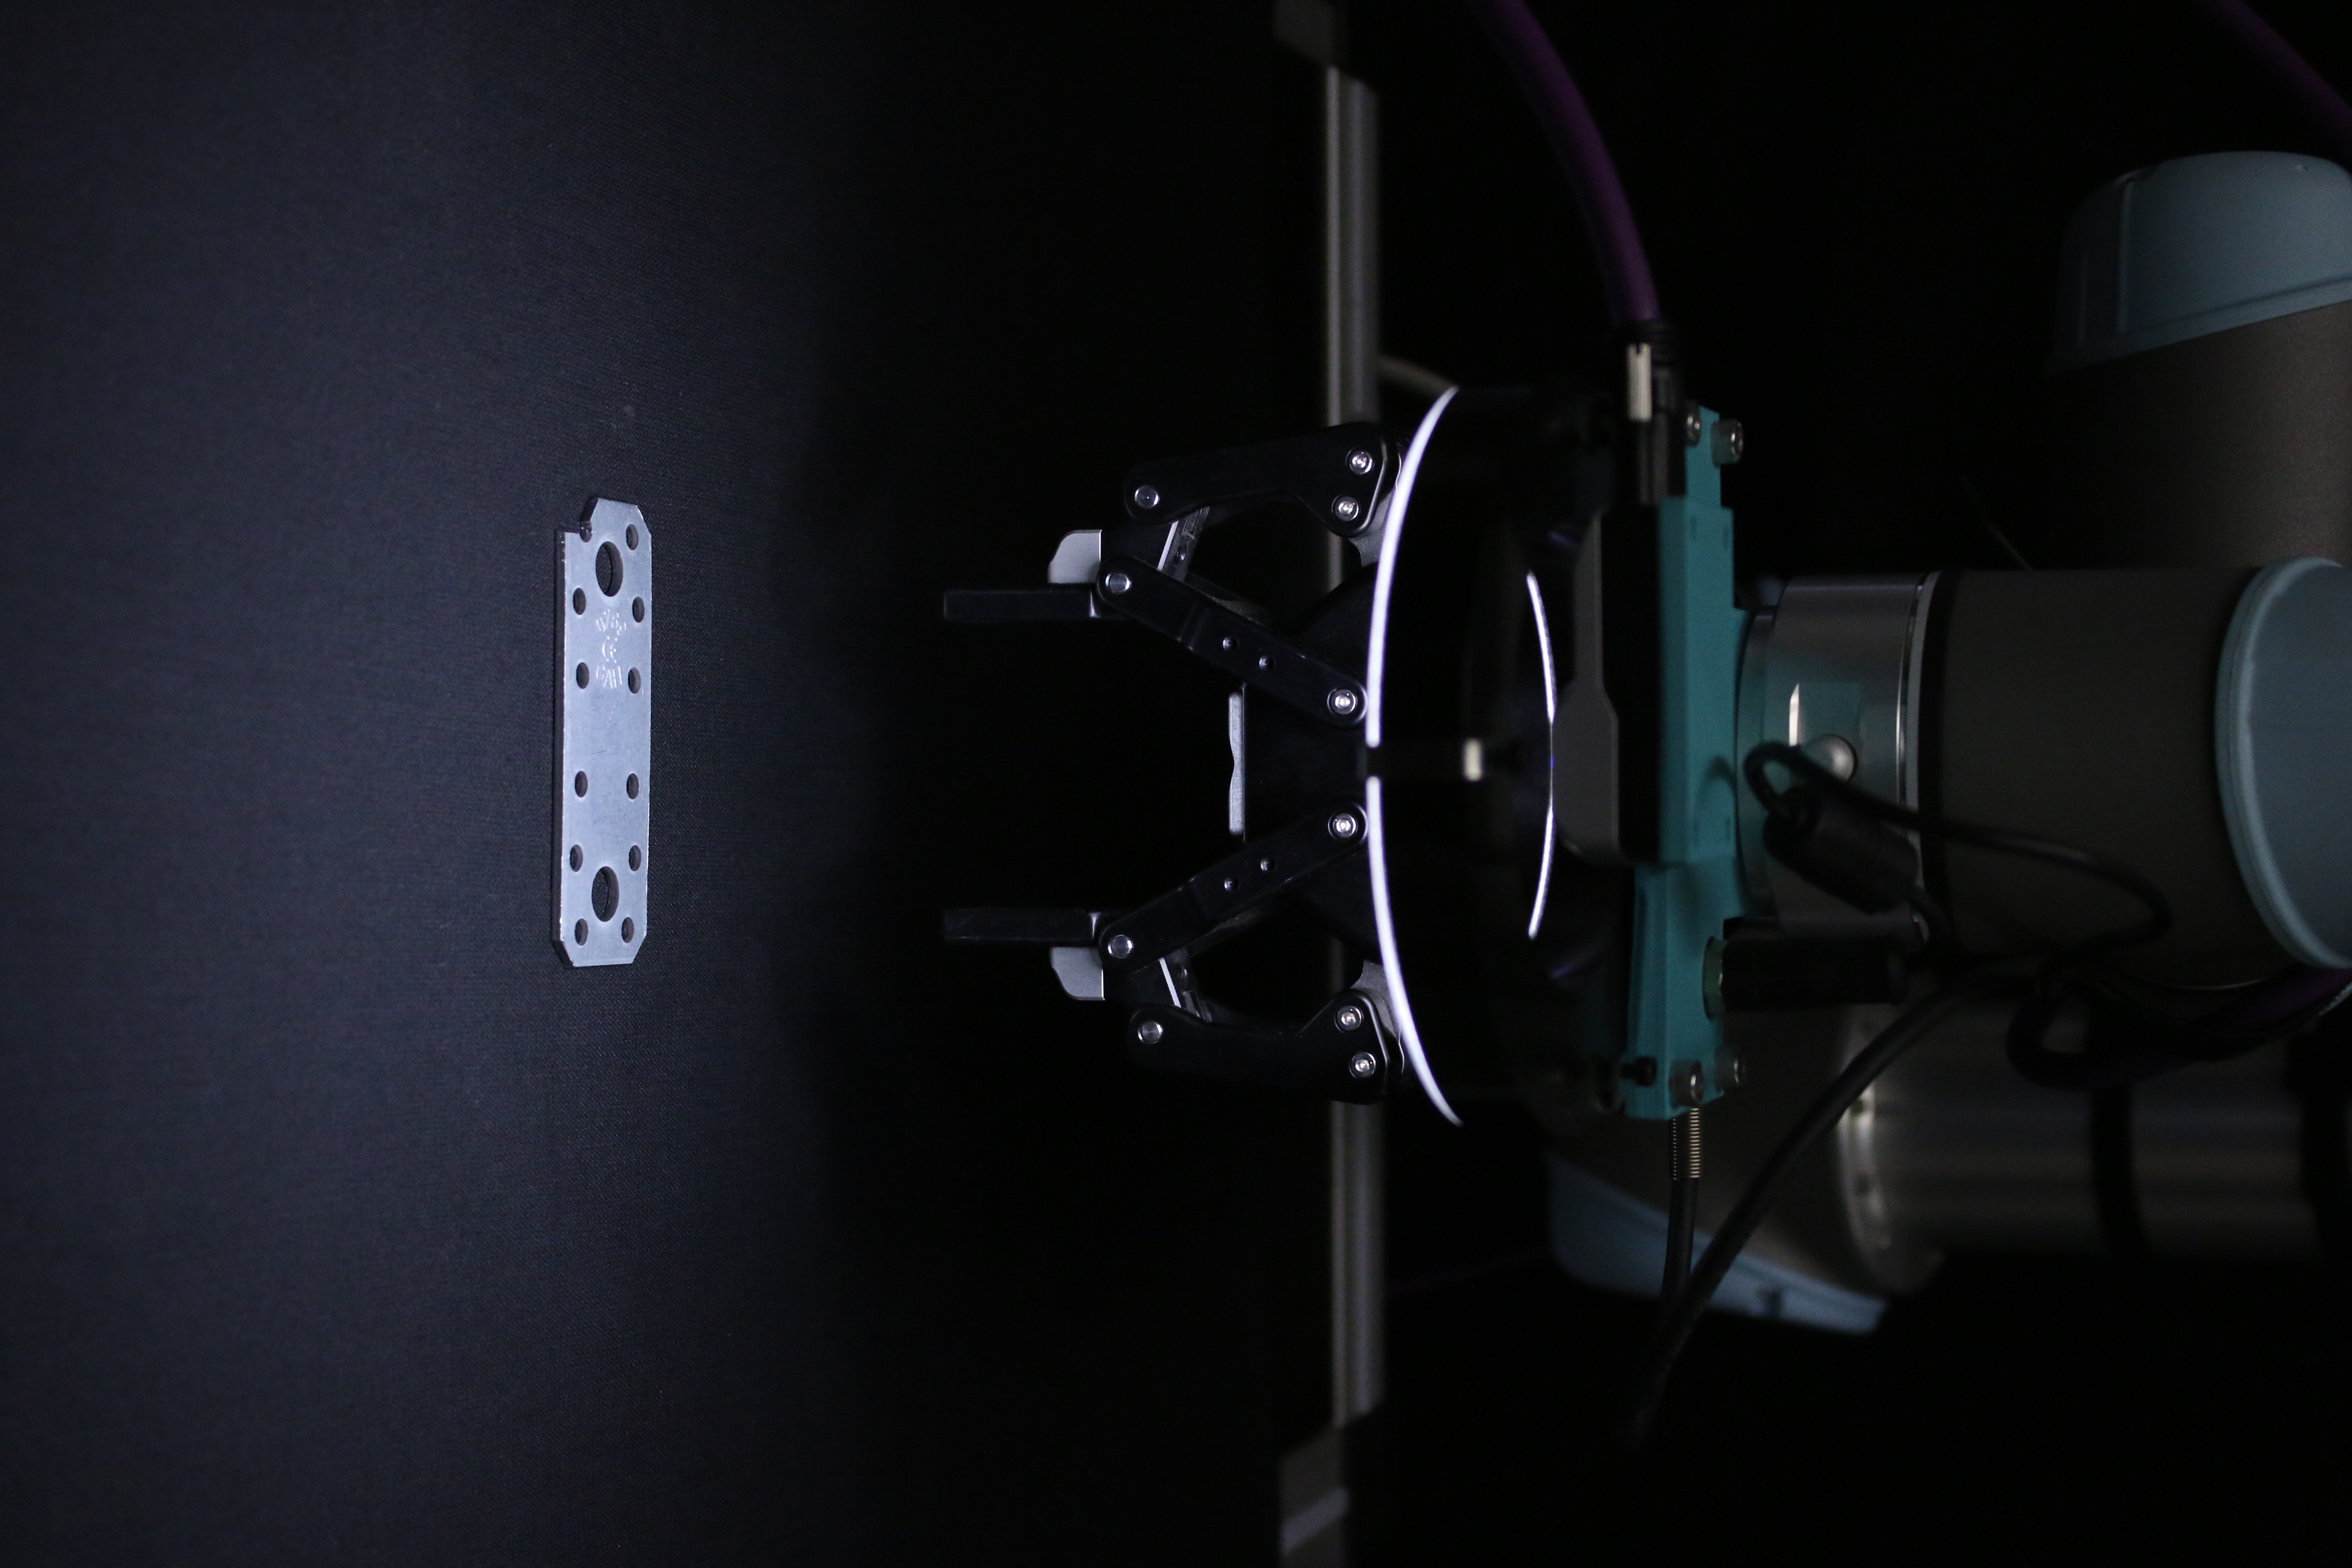
\includegraphics[angle=90, width=\textwidth]{figures/setupimages/setup_close.JPG}


    \end{subfigure}
    \caption{Images of the Environment of Data Collection}
    \label{fig:setupofdatacollection}
\end{figure}




\section{Anomalies}
\label{sec:flatconnectoranomalies}

To a certain degree, the standard MVTecAD LOCO classes all possess a balanced number of logical and structural anomalies. Therefore, the collection of possible anomalies for this class was kept at an even structural-to-logical ratio. The anomalies listed below can be viewed in Fig. \ref{fig:flatconnectorexampleimages}, where exemplary anomalous images are displayed next to their corresponding ground truth mask.

\subsection{Structural Anomalies}
Structural anomalies, in this case, were comparably simple to think of and execute since they only involved damaging some area of the flat connector. Here, we also tried to represent a variety of 
certain characteristics of anomalies among the ones we chose. An example would be to include anomalies with larger areas as well as ones with small ground truths.\newline
First, we produced the structural anomaly of a cut-off corner. This was done using a metal saw to remove a corner of the flat connector. This is an anomaly with a comparably large 
surface area and clean edges to predict. Next, we used a metal saw to damage the edges of the flat connector by cutting out pieces or simply sawing into the object's edges. One image 
of this anomaly type contained multiple damaged spots on multiple edges. Due to the cuts partially being tiny, this makes for an anomaly with very small ground truth areas, as seen in the Fig. 
\ref{fig:damagededgesubfig}. As a last structural anomaly, the saw was used to apply deep scratches to the object. This is mimicking another type of anomaly sometimes found in the classes of splicing connectors and pushpins 
in the original dataset. The common characteristic is that the region is very slim and long, making for better comparisons.

\subsection{Logical Anomalies}
The logical anomalies comprise the more relevant part of the anomaly types, as they are the focus of the MVTecAD LCOO dataset. The first logical anomaly in this class is the case in which a hole 
is missing in the flat connector hole pattern. This anomaly had to be improvised since it was difficult to obtain an adequately manufactured flat connector that was faulty. To still include 
this type of anomaly, the solution was first to fill the hole with moldable material and then spray paint over it to hide color differences. For realism, the spray paint color was the same as the 
object surface and the whole object was spray painted to avoid color artifacts. Partially, this anomaly was one of the larger and more clean-cut ones since the holes mostly chosen to be filled were one of the two 
bigger ones on the object. For increased variety, anomalous cases were also added where a small hole would be concealed. As a second anomaly, an extra hole was realized. To produce such an anomaly, the facilities offered a drill, which was used to drill another small hole into 
the object at an unusual location. The size of the additional hole was the same as the smaller ones on the object. To also test the capabilities of detecting multiple anomalies in a single image, this anomaly 
was put together with a differently-sized hole. The final anomaly to be introduced was a resized hole at a correct 
location. This would mean that the anomaly does not consist of the hole location but rather the size difference between these holes and those in similar places. For this type of anomaly, it 
is admissible to predict the whole hole as an anomalous region.
Here, a drill tip with a slightly higher radius than the original hole was used to enlarge the diameter.


\subsection{Saturation Thresholds}

The saturation scores for the anomalies, as discussed in section \ref{sec:datasets}, were put at the number of pixels in the anomalous region for all the listed anomalies, 
respectively.
This was because the nature of the presented anomalies of these categories calls for a complete segmentation of the respective anomaly for a perfect result. Unlike in the pushpin example given in that section 
there are no cases that warrant multiple possible placements of anomalies.






